\documentclass[enabledeprecatedfontcommands,fontsize=12pt,paper=a4,twoside]{scrartcl}


\newcommand{\grad}{\ensuremath{^{\circ}} }
\renewcommand{\strut}{\vrule width 0pt height5mm depth2mm}

\usepackage{longtable}
\usepackage[utf8]{inputenc}
\usepackage[T1]{fontenc}
\usepackage[final]{pdfpages}
% obere Seitenränder gestalten können
\usepackage{fancyhdr}
\usepackage{moreverb}
% Graphiken als jpg, png etc. einbinden können
\usepackage{graphicx}
\usepackage[normalem]{ulem}
\useunder{\uline}{\ul}{}
\usepackage{stmaryrd}
% Floats Objekte mit [H] festsetzen
\usepackage{float}
% setzt URL's schön mit \url{http://bla.laber.com/~mypage}
\usepackage{url}
% Externe PDF's einbinden können
\usepackage{pdflscape}
% Verweise innerhalb des Dokuments schick mit " ... auf Seite ... "
% automatisch versehen. Dazu \vref{labelname} benutzen
\usepackage[ngerman]{varioref}
\usepackage[ngerman]{babel}
\usepackage{ngerman}
% Bibliographie
\usepackage{bibgerm}
% Tabellen
\usepackage{tabularx}
\usepackage{supertabular}
\usepackage[colorlinks=true, pdfstartview=FitV, linkcolor=blue,
            citecolor=blue, urlcolor=blue, hyperfigures=true,
            pdftex=true]{hyperref}
\usepackage{bookmark}
\usepackage{rotating}
\usepackage{float}
\usepackage{hyperref}

\hyphenation{Arbeits-paket}

% Damit Latex nicht zu lange Zeilen produziert:
\sloppy
%Uneinheitlicher unterer Seitenrand:
%\raggedbottom

% Kein Erstzeileneinzug beim Absatzanfang
% Sieht aber nur gut aus, wenn man zwischen Absätzen viel Platz einbaut
\setlength{\parindent}{0ex}

% Abstand zwischen zwei Absätzen
\setlength{\parskip}{1ex}

% Seitenränder für Korrekturen verändern
\addtolength{\evensidemargin}{-1cm}
\addtolength{\oddsidemargin}{1cm}

\bibliographystyle{gerapali}

% Lustige Header auf den Seiten
  \pagestyle{fancy}
  \setlength{\headheight}{70.55003pt}
  \fancyhead{}
  \fancyhead[LO,RE]{Software--Projekt 2\\ WiSe 2019/2020
  \\Architekturbeschreibung}
  \fancyhead[LE,RO]{Seite \thepage\\\slshape \leftmark\\\slshape \rightmark}

%Unicode Minuszeichen deklarieren, um es nicht überall austauschen zu müssen
\DeclareUnicodeCharacter{2212}{-}

%
% Und jetzt geht das Dokument los....
%

\begin{document}

% Lustige Header nur auf dieser Seite
  \thispagestyle{fancy}
  \fancyhead[LO,RE]{ }
  \fancyhead[LE,RO]{Universität Bremen\\FB 3 -- Informatik\\
  Prof. Dr. Rainer Koschke \\TutorIn: Marcel Steinbeck}
  \fancyfoot[C]{}

% Start Titelseite
  \vspace{3cm}

  \begin{minipage}[H]{\textwidth}
  \begin{center}
  \bf
  \Large
  Software--Projekt 2 WiSe 2019/2020\\
  \smallskip
  \small
  VAK 03-BA-901.02\\
  \vspace{3cm}
  \end{center}
  \end{minipage}
  \begin{minipage}[H]{\textwidth}
  \begin{center}
  \vspace{1cm}
  \bf
  \Large Testprotokoll\\ Data Colorado\\
  \vfill
  \end{center}
  \centering
  
\includegraphics[width=0.4\textwidth]{Bilder/Logo.png}\\
  \end{minipage}
  \vfill
  \begin{minipage}[H]{\textwidth}
  \begin{center}
  \sf
  \begin{tabular}{lr}
  Liam Hurwitz & hurwitz@tzi.de \\
  Kevin Santiago Rodriguez Rey & kev\textunderscore rey@tzi.de \\
  Fabian Kehlenbeck & fkehlenb@tzi.de \\
  Aaron Rudkowski & rudkowsk@tzi.de \\
  Samuel Nejati Masouleh & samnej@tzi.de \\
  Leonard Haddad & s\textunderscore xsipo6@tzi.de \\  
\end{tabular}
  \\ ~
  \vspace{2cm}
  \\
  \it Abgabe: 08.03.2020 --- Version 1.0\\ ~
  \end{center}
  \end{minipage}

% Ende Titelseite

% Start Leerseite

\newpage

  \thispagestyle{fancy}
  \fancyhead{}
  \fancyhead[LO,RE]{Software--Projekt \\  2019/2020
  \\Benutzerhandbuch}
  \fancyhead[LE,RO]{Seite \thepage\\\slshape \leftmark\\~}
  \fancyfoot{}
  \renewcommand{\headrulewidth}{0.4pt}
  \tableofcontents

\newpage

  \fancyhead[LE,RO]{Seite \thepage\\\slshape \leftmark\\\slshape \rightmark}


%%%%%%%%%%%%%%%%%%%%%%%%%%%%%%%%%%%%%%%%%%%%%%%%%%%%%%%%%%%%%%%%%%%%%%%%


\section*{Version und Änderungsgeschichte}

{\em Die aktuelle Versionsnummer des Dokumentes sollte eindeutig und gut zu
identifizieren sein, hier und optimalerweise auf dem Titelblatt.}

\begin{tabular}{ccl}
Version & Datum & Änderungen \\
\hline
%0.1 & TT.MM.JJJJ & Dokumentvorlage als initiale Fassung kopiert \\
0.1 & 03.03.2020 & Erste Schritte \\
0.2 & 03.03.2020 & Administrator \\
\end{tabular}


%%%%%%%%%%%%%%%%%%%%%%%%%%%%%%%%%%%%%%%%%%%%%%%%%%%%%%%%%%%%%%%%%%%%%%%%

\newpage
\section{Einführung}

%%%%%%%%%%%%%%%%%%%%%%%%%%%%%%%%%%%%%%%%%%%%%%%%%%%%%%%%%%%%%%%%%%%%%%%%

\newpage
\section{Übersicht}

%%%%%%%%%%%%%%%%%%%%%%%%%%%%%%%%%%%%%%%%%%%%%%%%%%%%%%%%%%%%%%%%%%%%%%%%

\newpage
\section{Tests}

\subsection{Tests zur Generellen Funktion}

\subsubsection{Anwendungsfall: Login unterschiedlicher Nutzer}

\textbf{Testvorbedingungen:} Sobald man die Webseite aufruft, wird man auf die \hyperlink{sc3.1.1.1}{Startseite}  geleitet. \\

\hypertarget{sc3.1.1.1}{
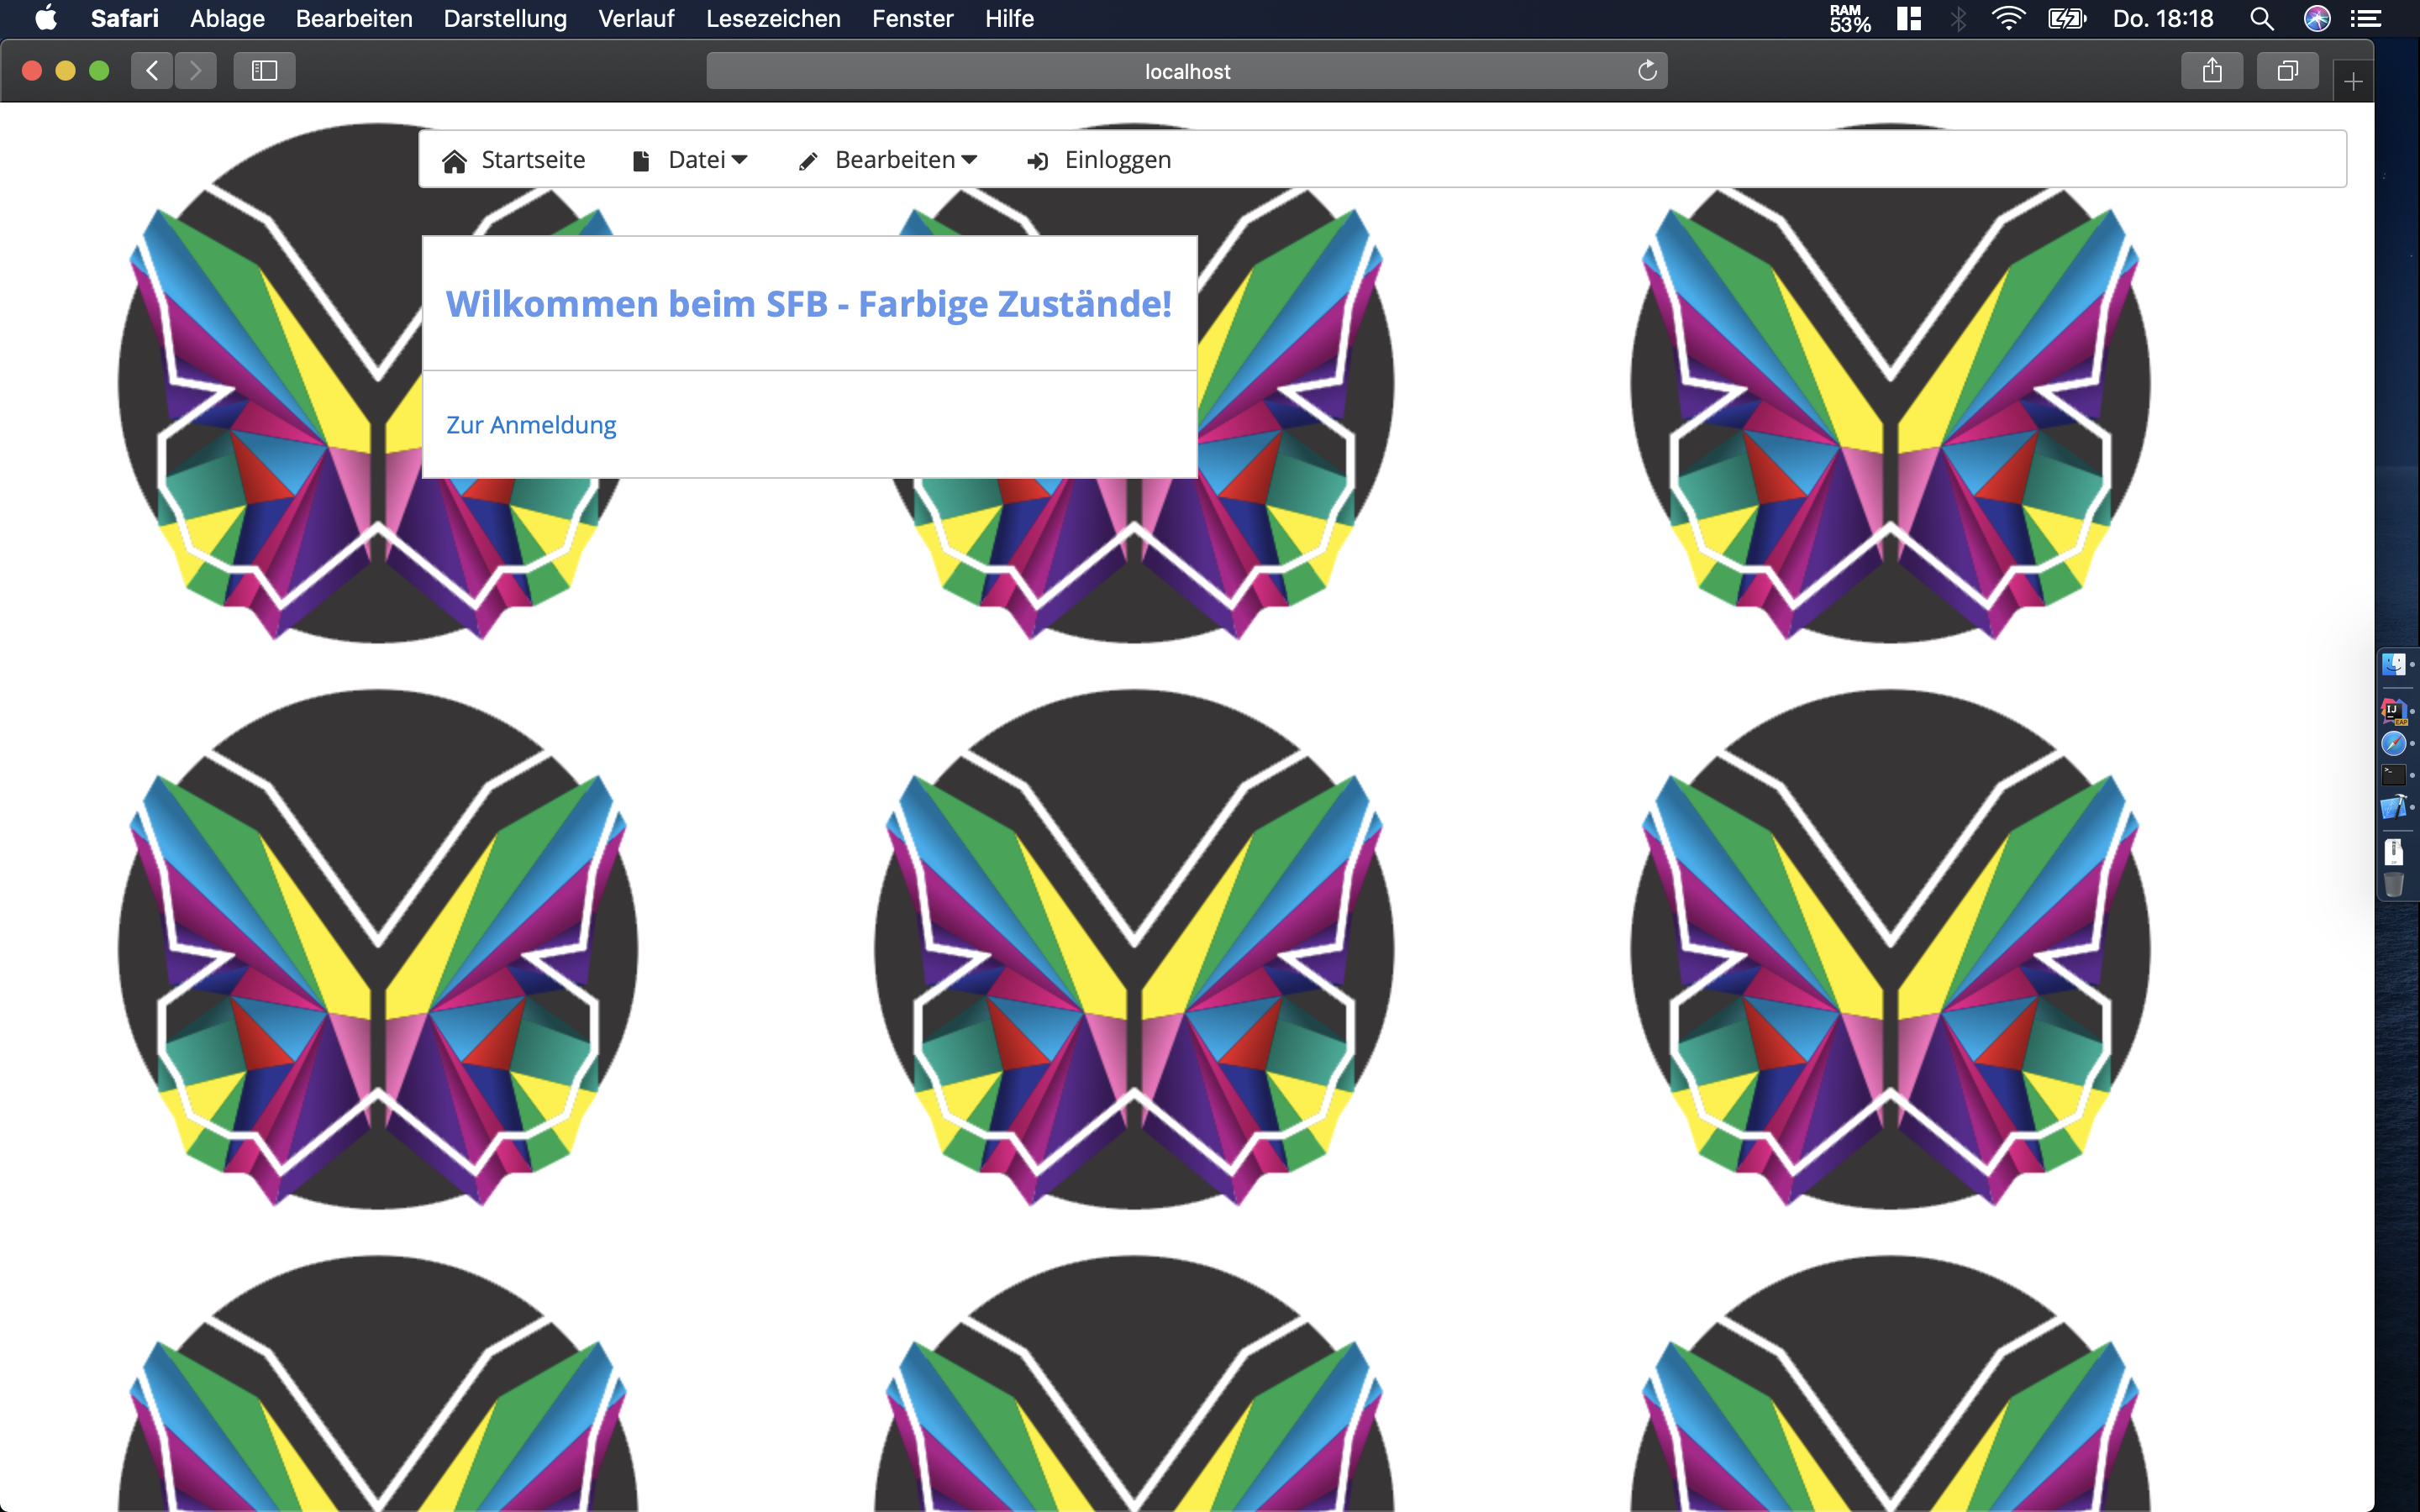
\includegraphics[width=1\textwidth]{Screenshots/311StartSite.png}
\textit{Abbildung 3.1.1.1: Startseite}
} \\

Hier kann man nun auf den Button \textit{Zur Anmeldung} drücken, um zur \hyperlink{sc3.1.1.2}{Loginseite} weitergeleitet zu werden. Ein valider Login ist der Benutzername \textit{admin} und das Passwort \textit{12345678}. \\

\hypertarget{sc3.1.1.2}{
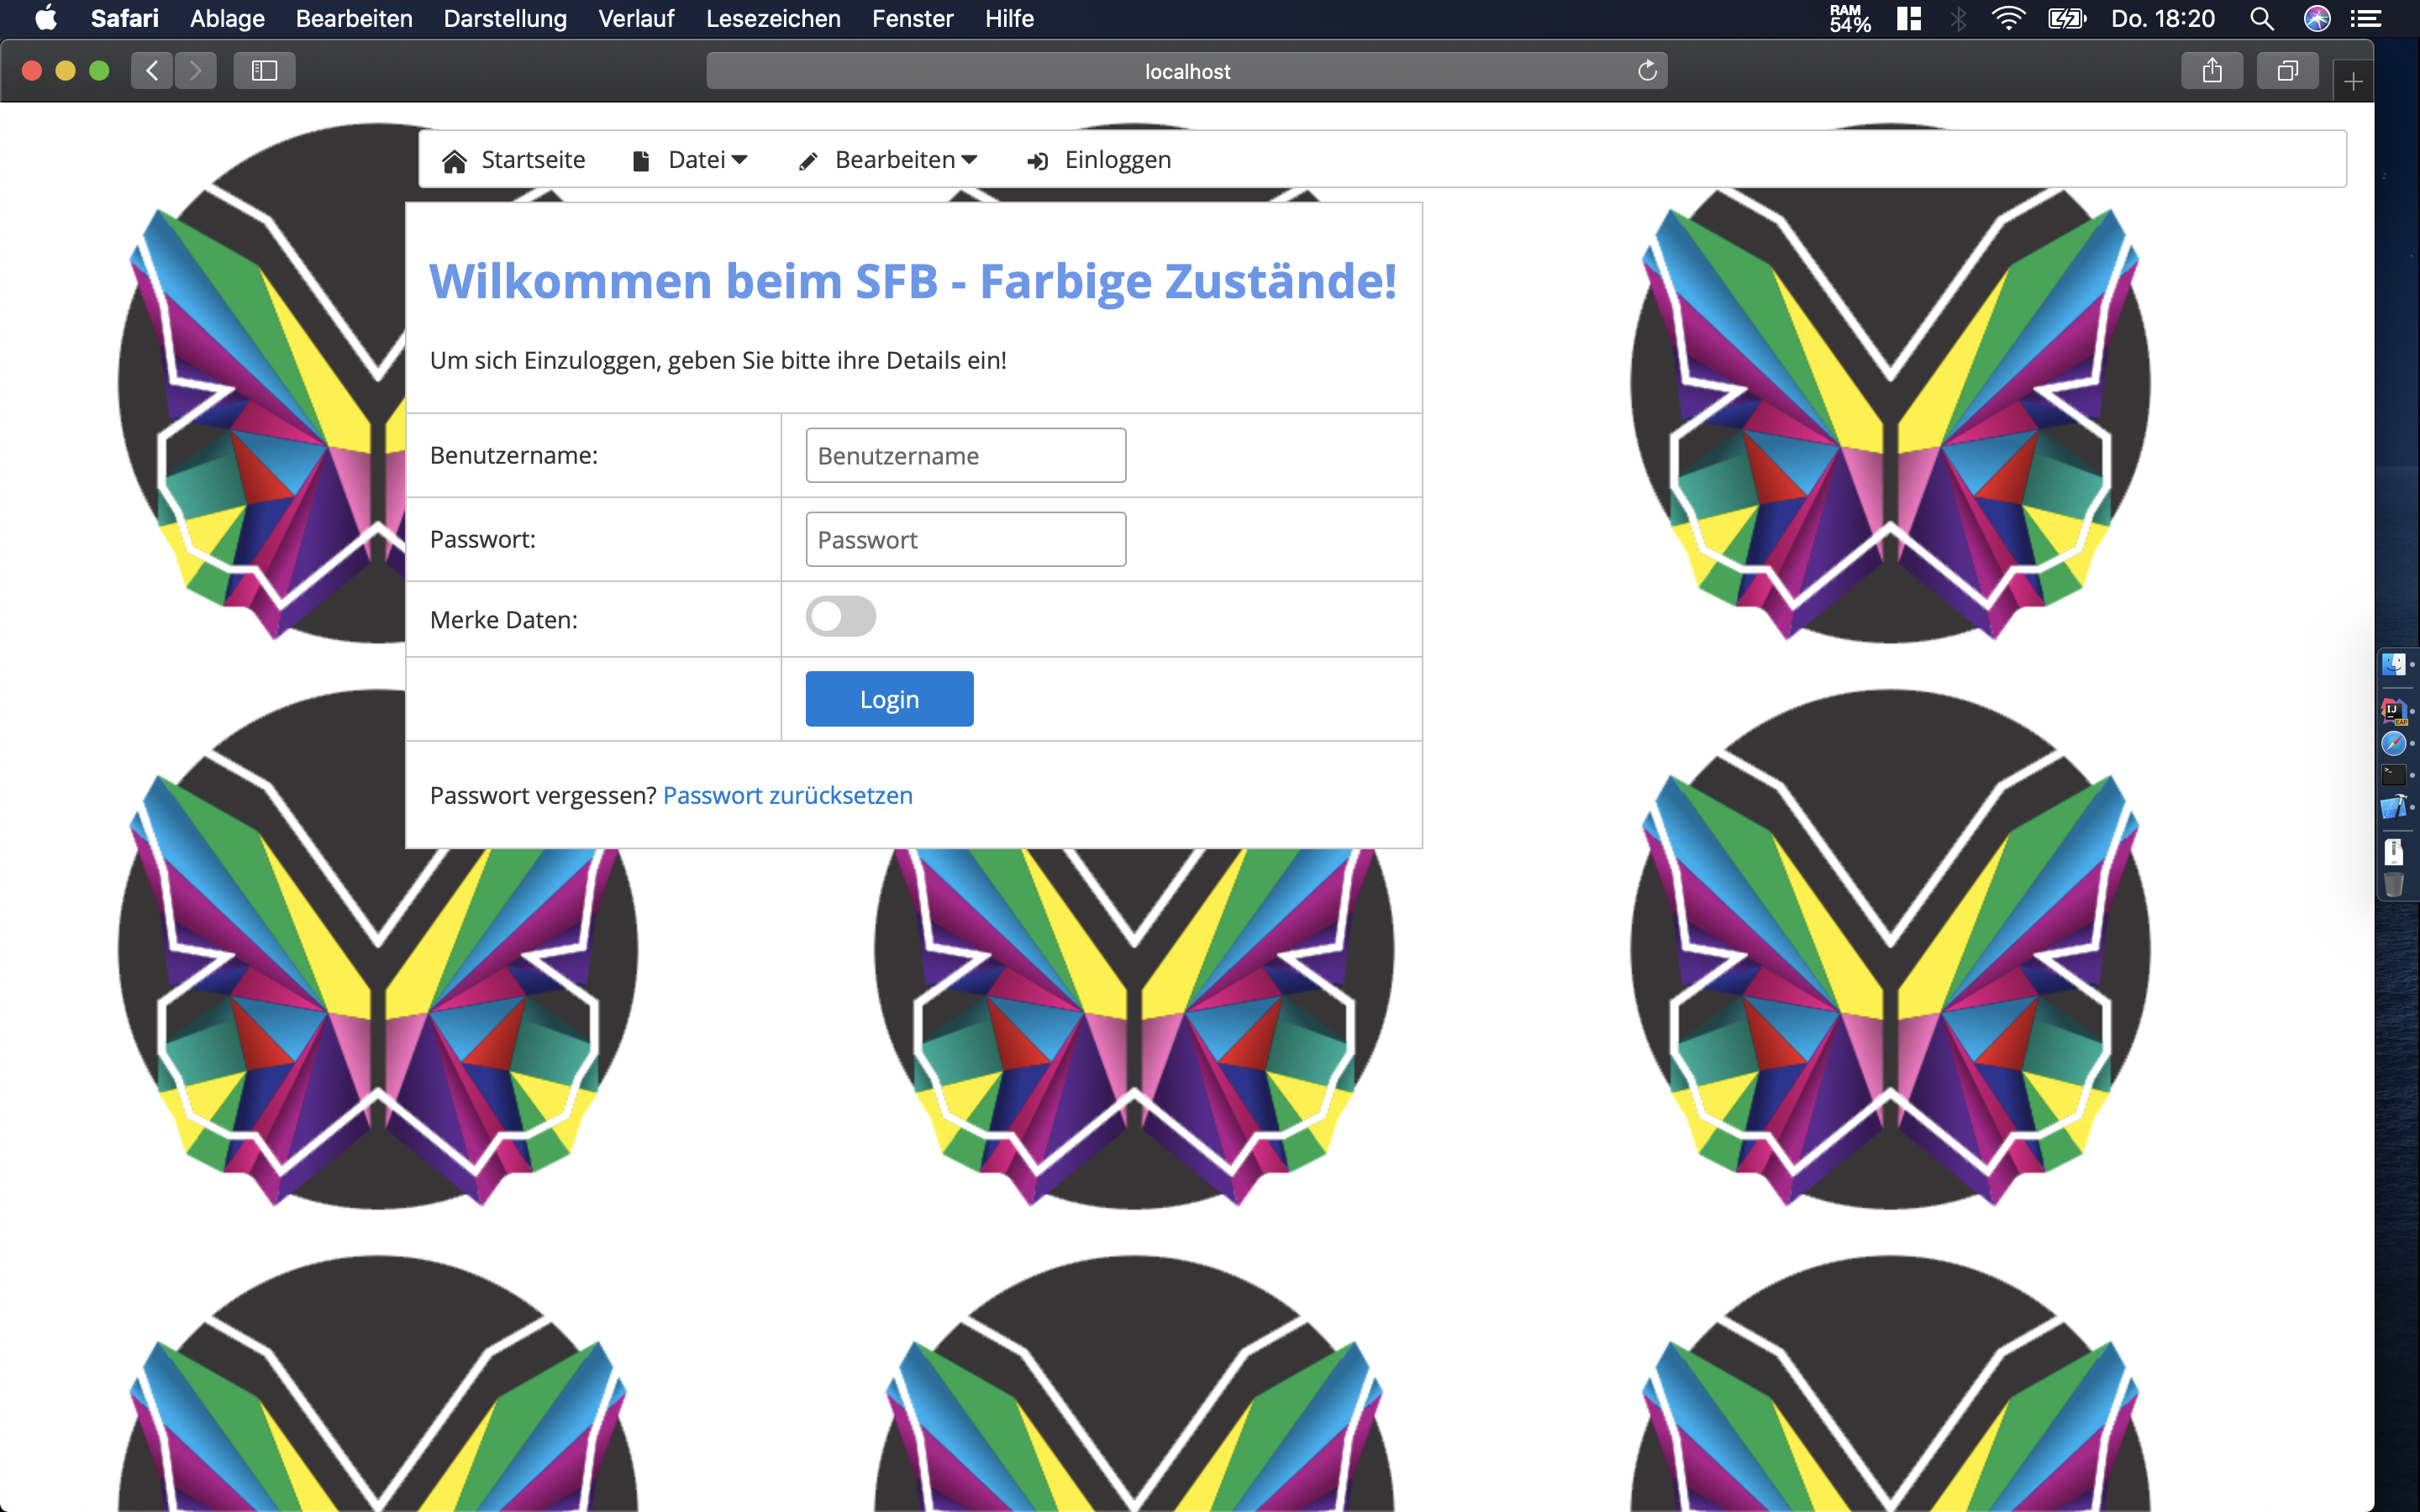
\includegraphics[width=1\textwidth]{Screenshots/311LoginSite.png}
\textit{Abbildung 3.1.1.2: Loginseite}
} \\

Jetzt haben wir uns als erstes mit einem falschen Passwort angemeldet, was eine Fehlermeldung wirft, wie man auf dem nächsten  \hyperlink{sc3.1.1.3}{Screenshot} in der oberen Ecke sieht.\\

\hypertarget{sc3.1.1.3}{
\includegraphics[width=1\textwidth]{Screenshots/311wrongPassword.png}
\textit{Abbildung 3.1.1.3: Falsches Passwort für Admin eingegeben}
} \\

Anschließend wurde versucht, sich mit den validen Logindaten des Admins einzuloggen und man kommt auf die \hyperlink{sc3.1.1.4}{Startseite des Admins}. \\

\hypertarget{sc3.1.1.4}{
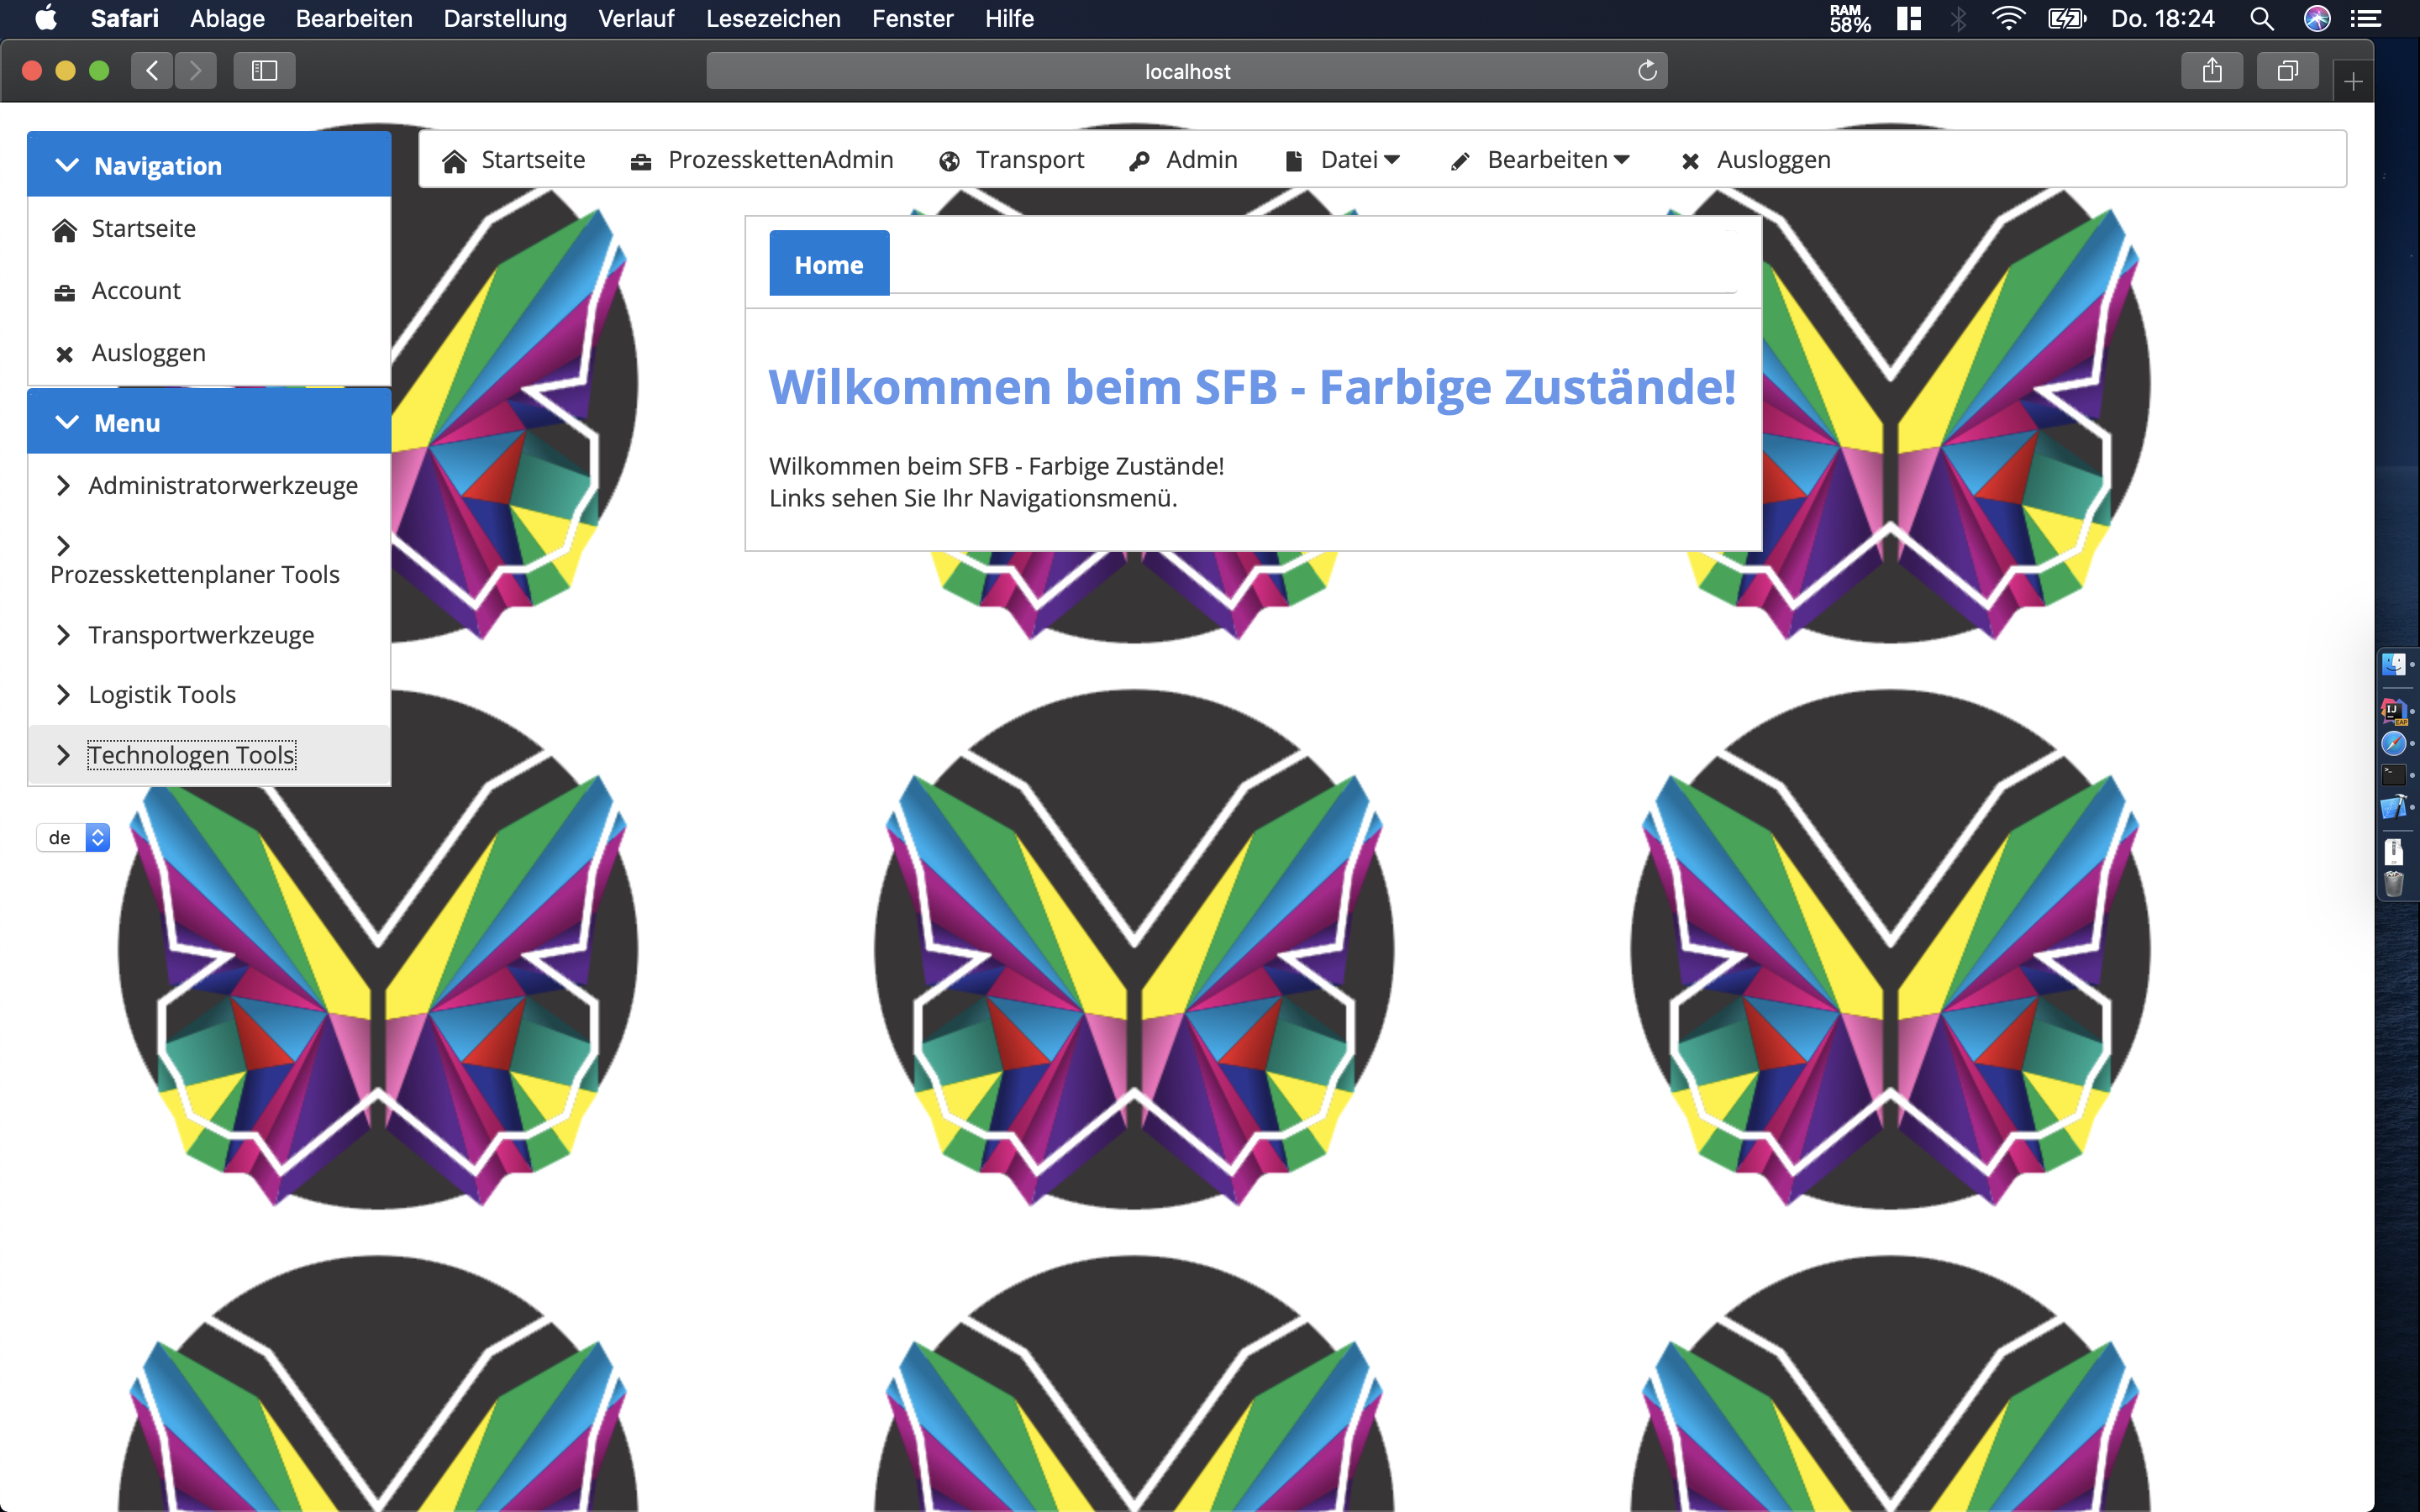
\includegraphics[width=1\textwidth]{Screenshots/311AdminView.png}
\textit{Abbildung 3.1.1.4: Richtiges Passwort für Admin eingegeben}
} \\

Jetzt wurde sich noch versucht, mit den validen Logindaten für den Technologen einzuloggen. Man wird auf die \hyperlink{sc3.1.1.5}{Startseite des Technologen} weitergeleitet. \\

\hypertarget{sc3.1.1.5}{
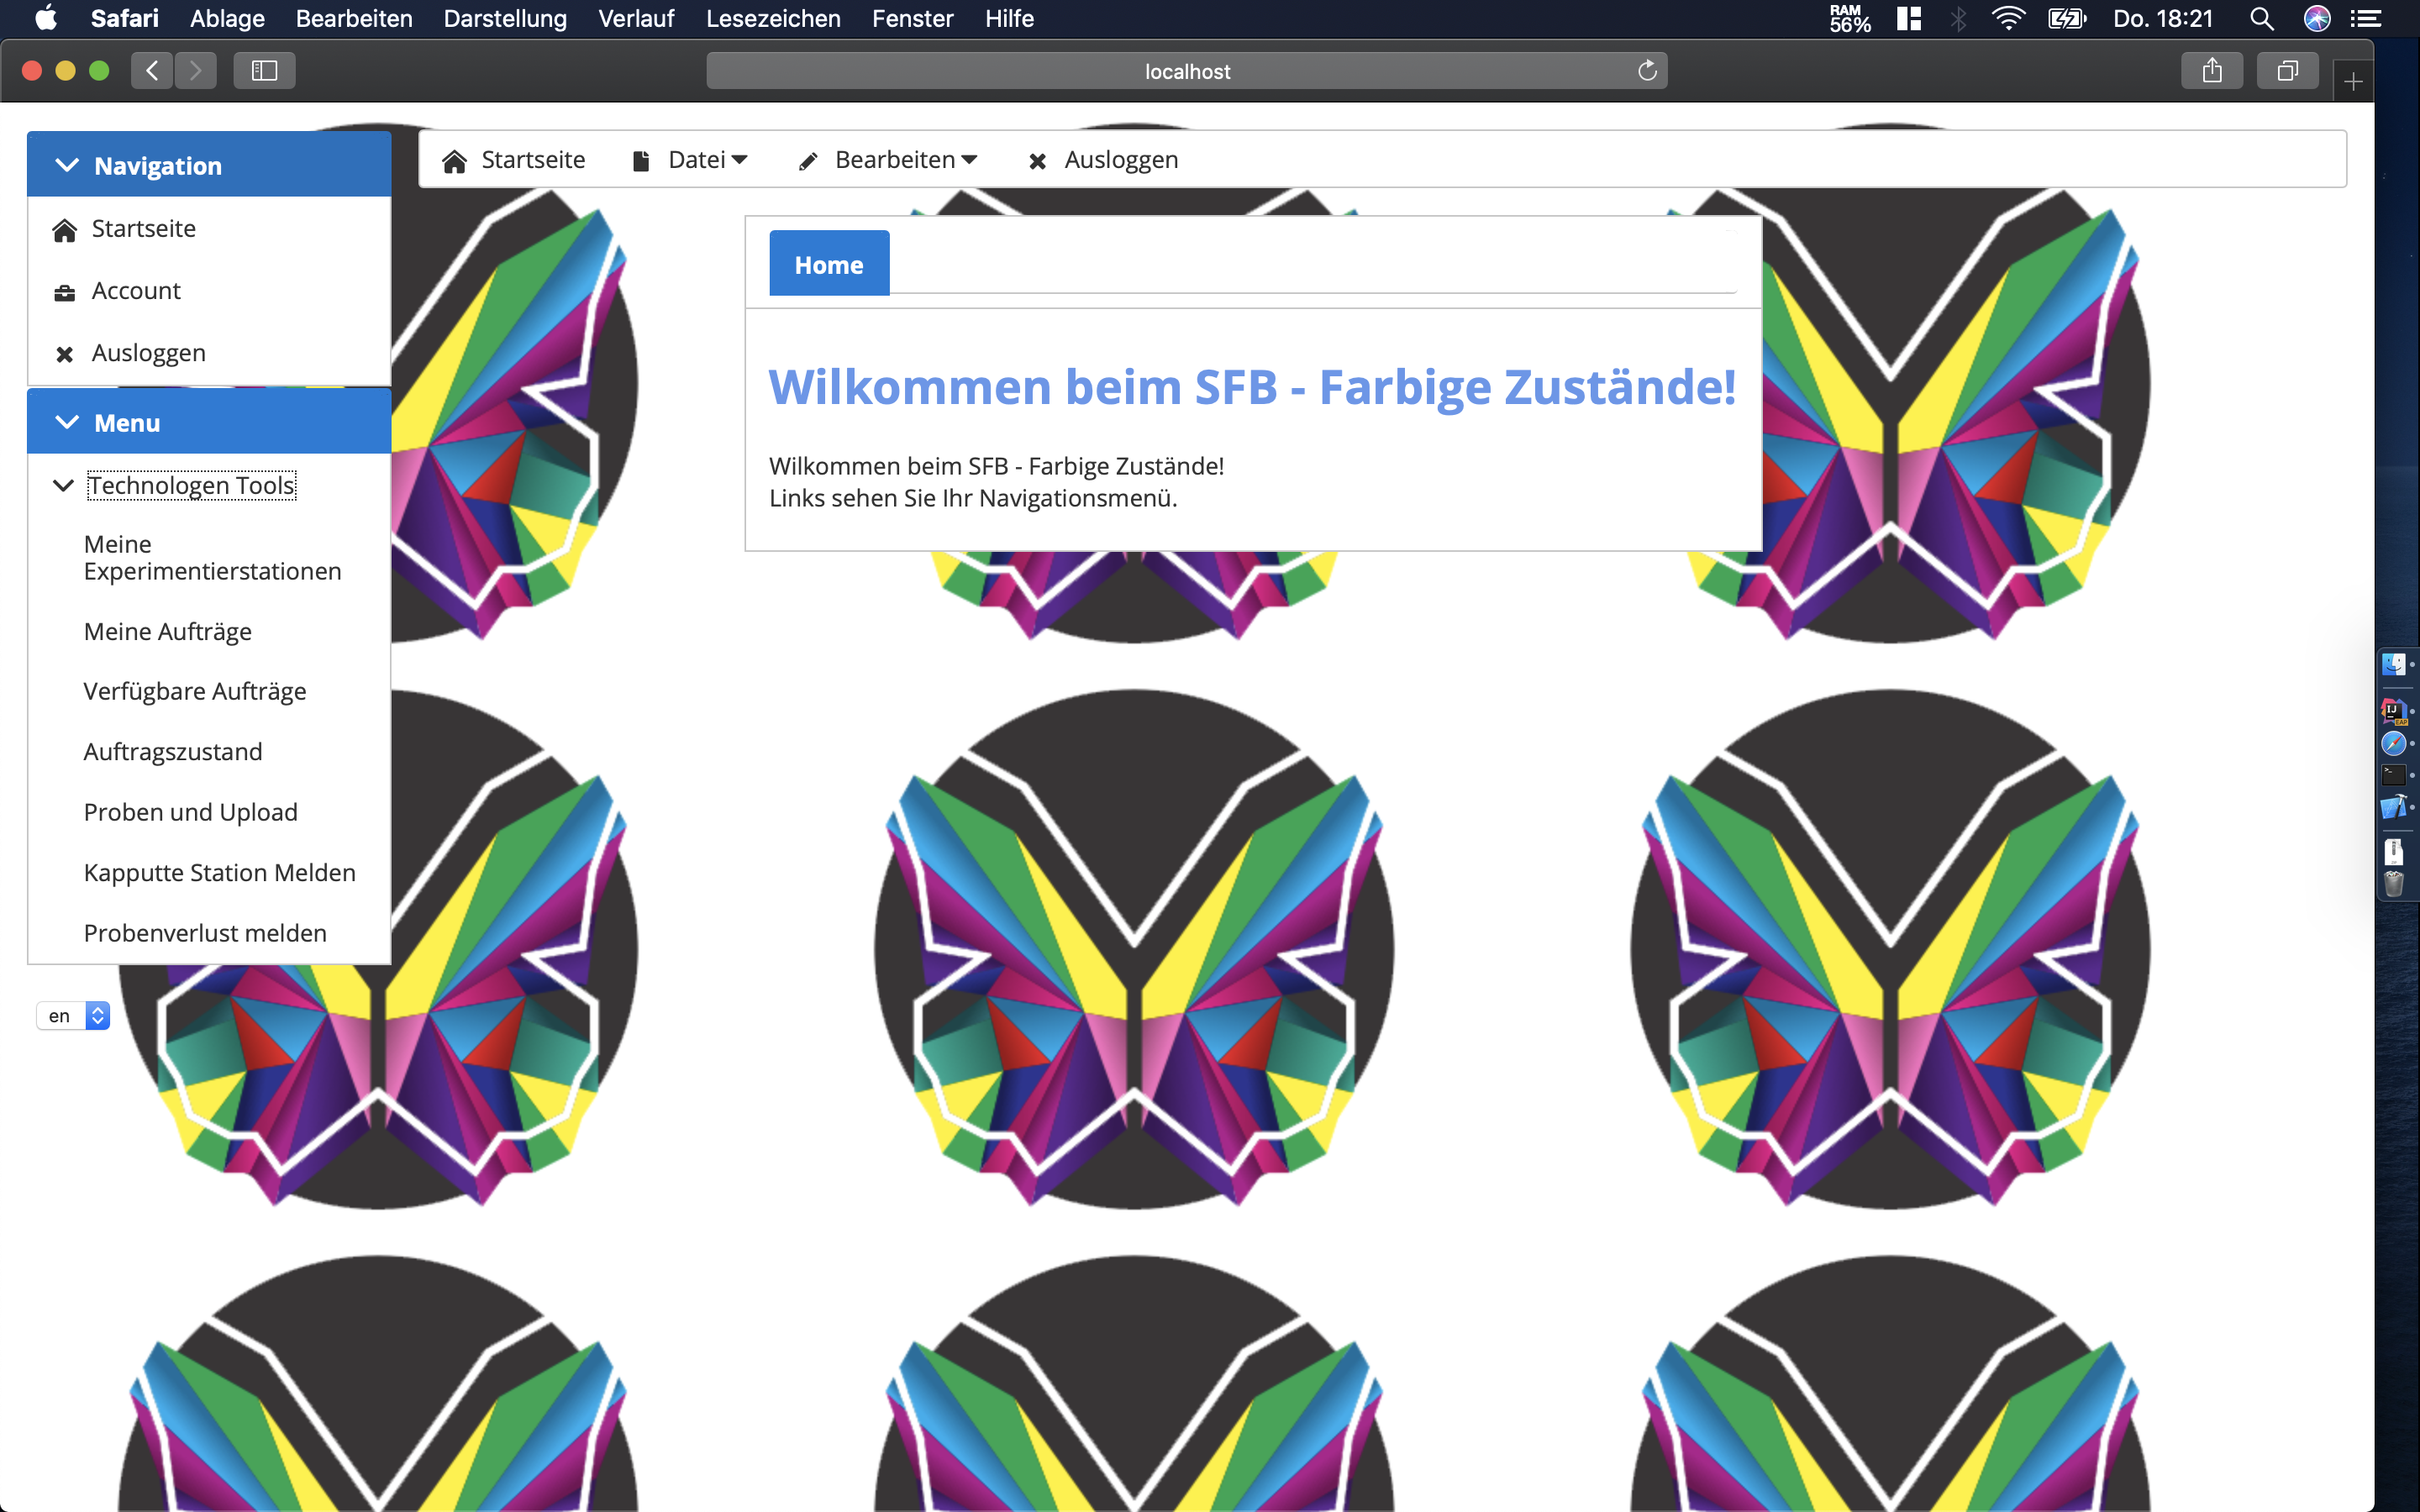
\includegraphics[width=1\textwidth]{Screenshots/311TechnologeView.png}
\textit{Abbildung 3.1.1.5: Richtiges Passwort für Technologen eingegeben}
} \\

Wie man in den Beispielen sehen kann, kann man sich mit unterschiedlichen Benutzern einloggen, welche unterschiedliche den Rollen entsprechende Features haben. Man muss das richtige Passwort für den Benutzernamen eingeben, um sich einloggen zu können. Die Tests verliefen erfolgreich. \\

%%Santiago gfeschrieben
An der Folgende Grafik kann man sehen die Fehlermeldungen, die man bekommt, durch Leer Textfelder an der Anmeldung Webseite.

\hypertarget{sc3.1.1.6}{
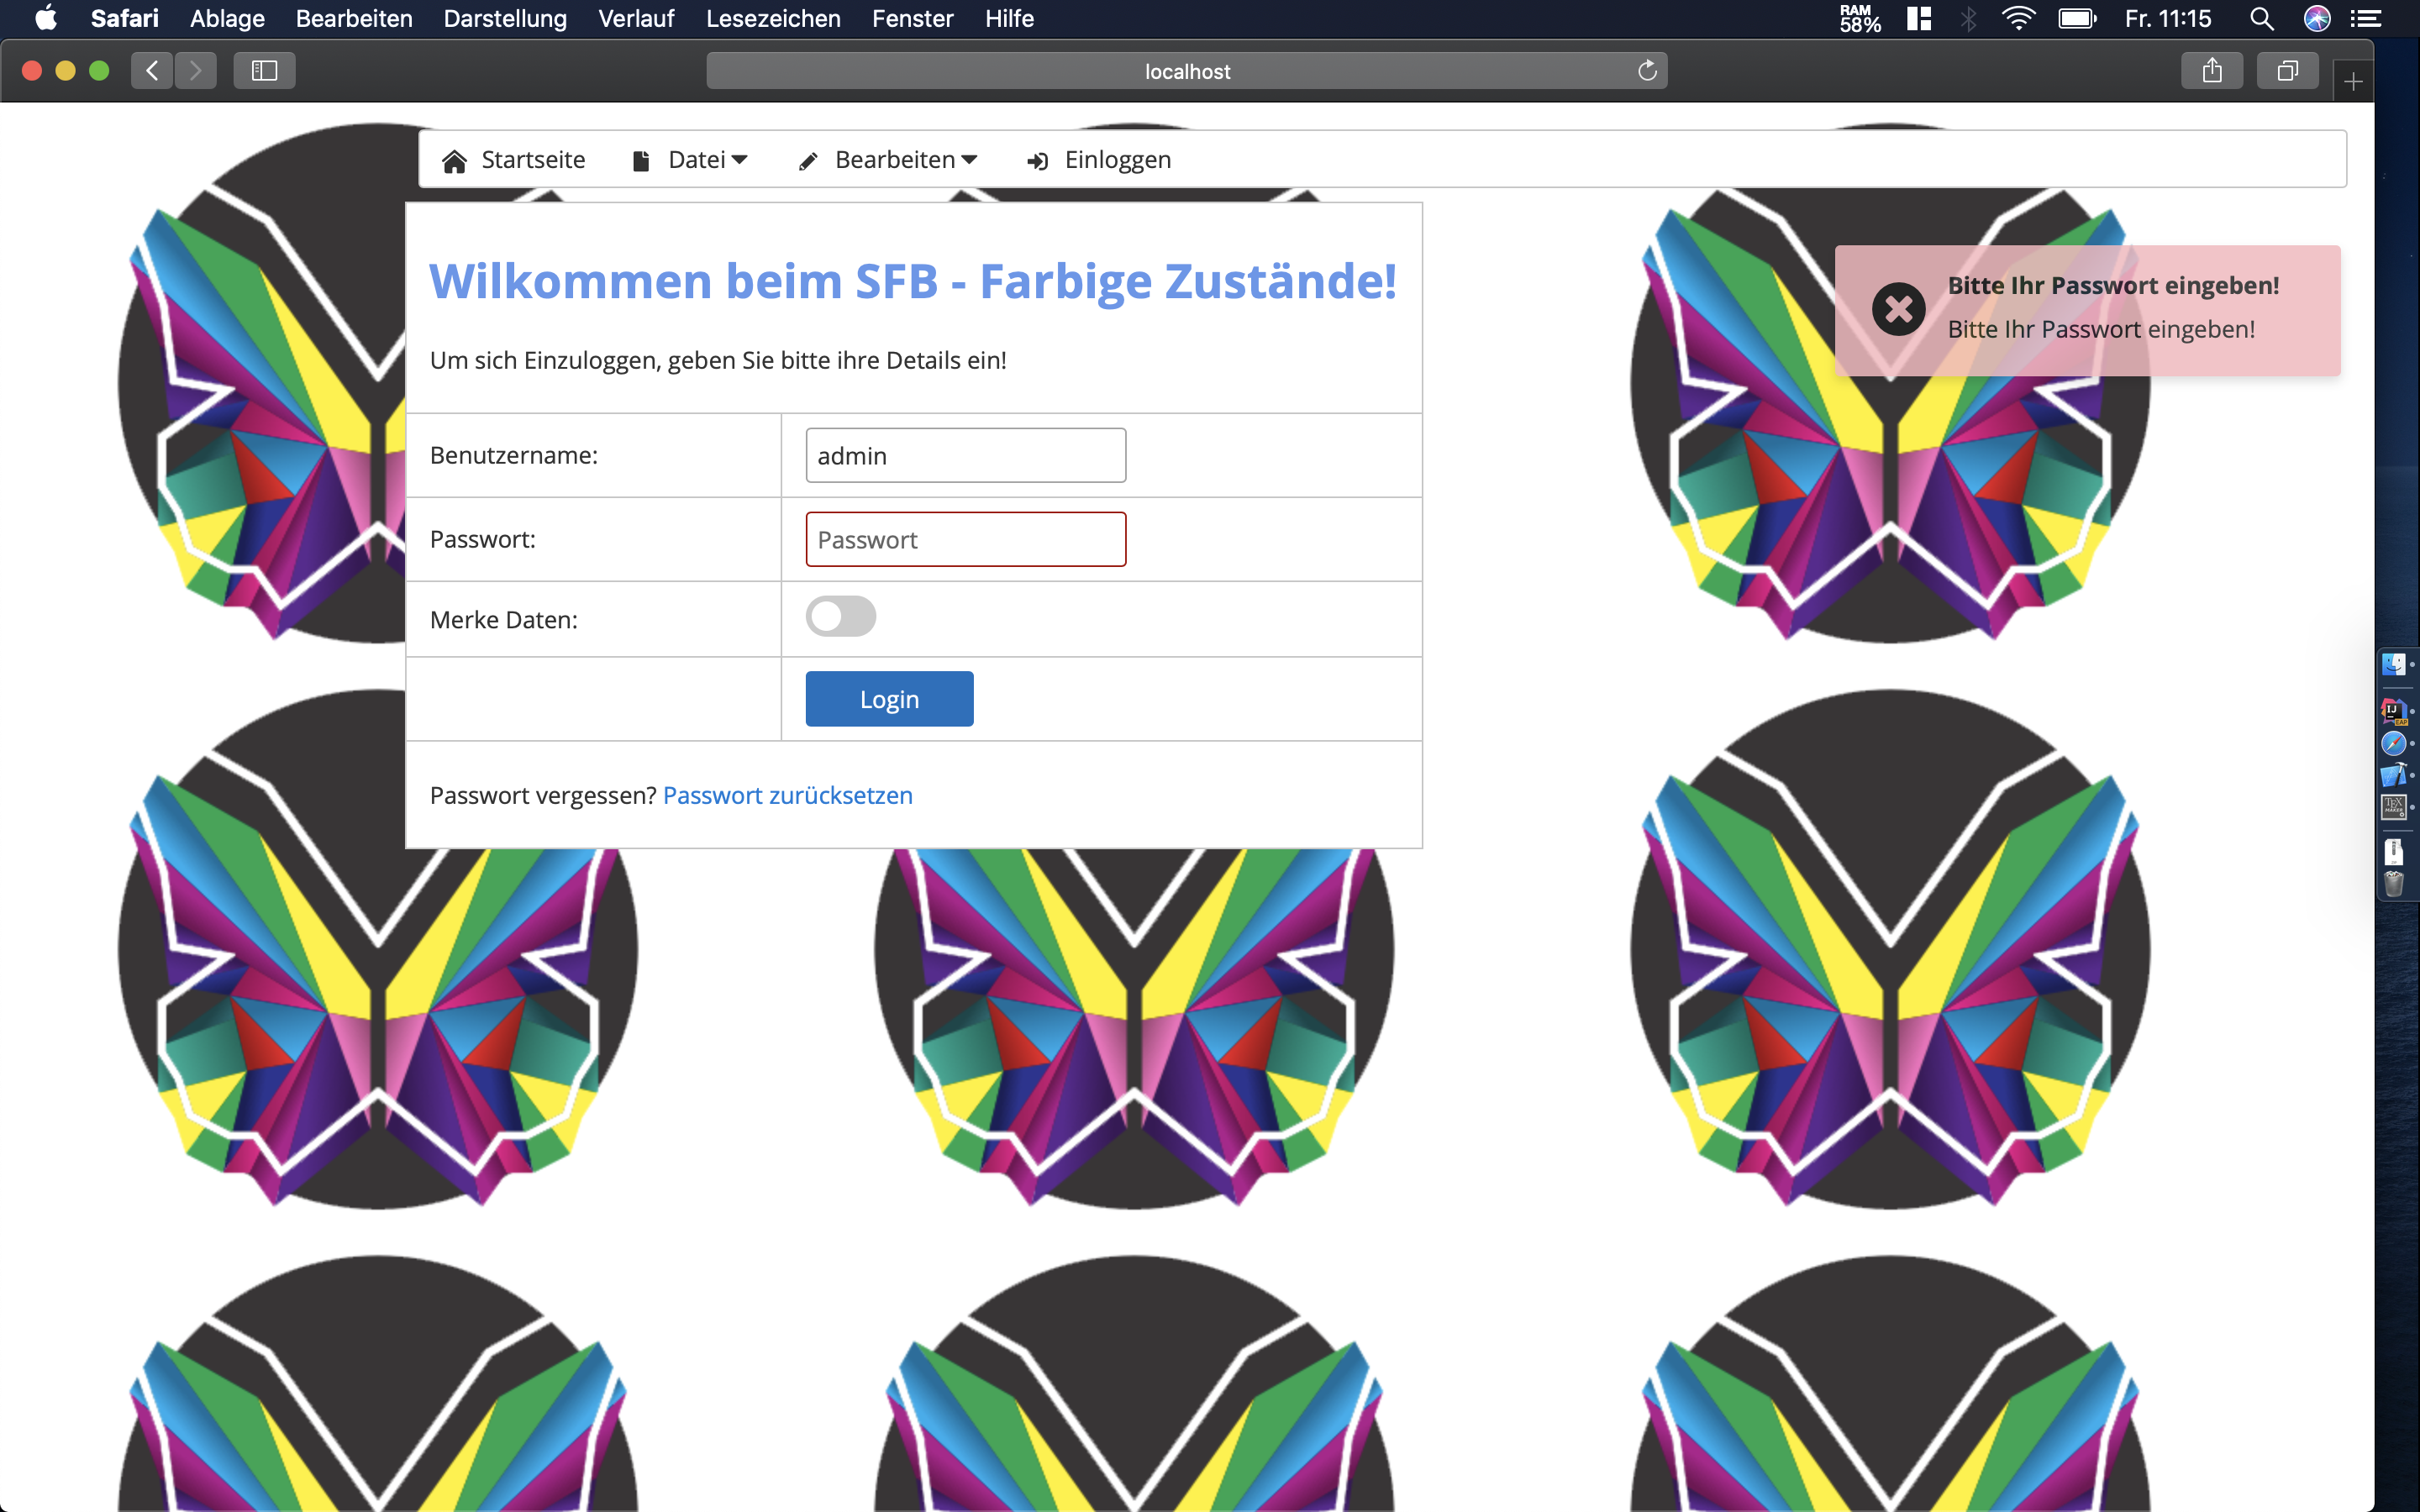
\includegraphics[width=1\textwidth]{Screenshots/311BittePasswordEingeben.png}\\ \textit{Abbildung 3.1.1.6: Benutzer ohne password}
} \\

\hypertarget{sc3.1.1.7}{
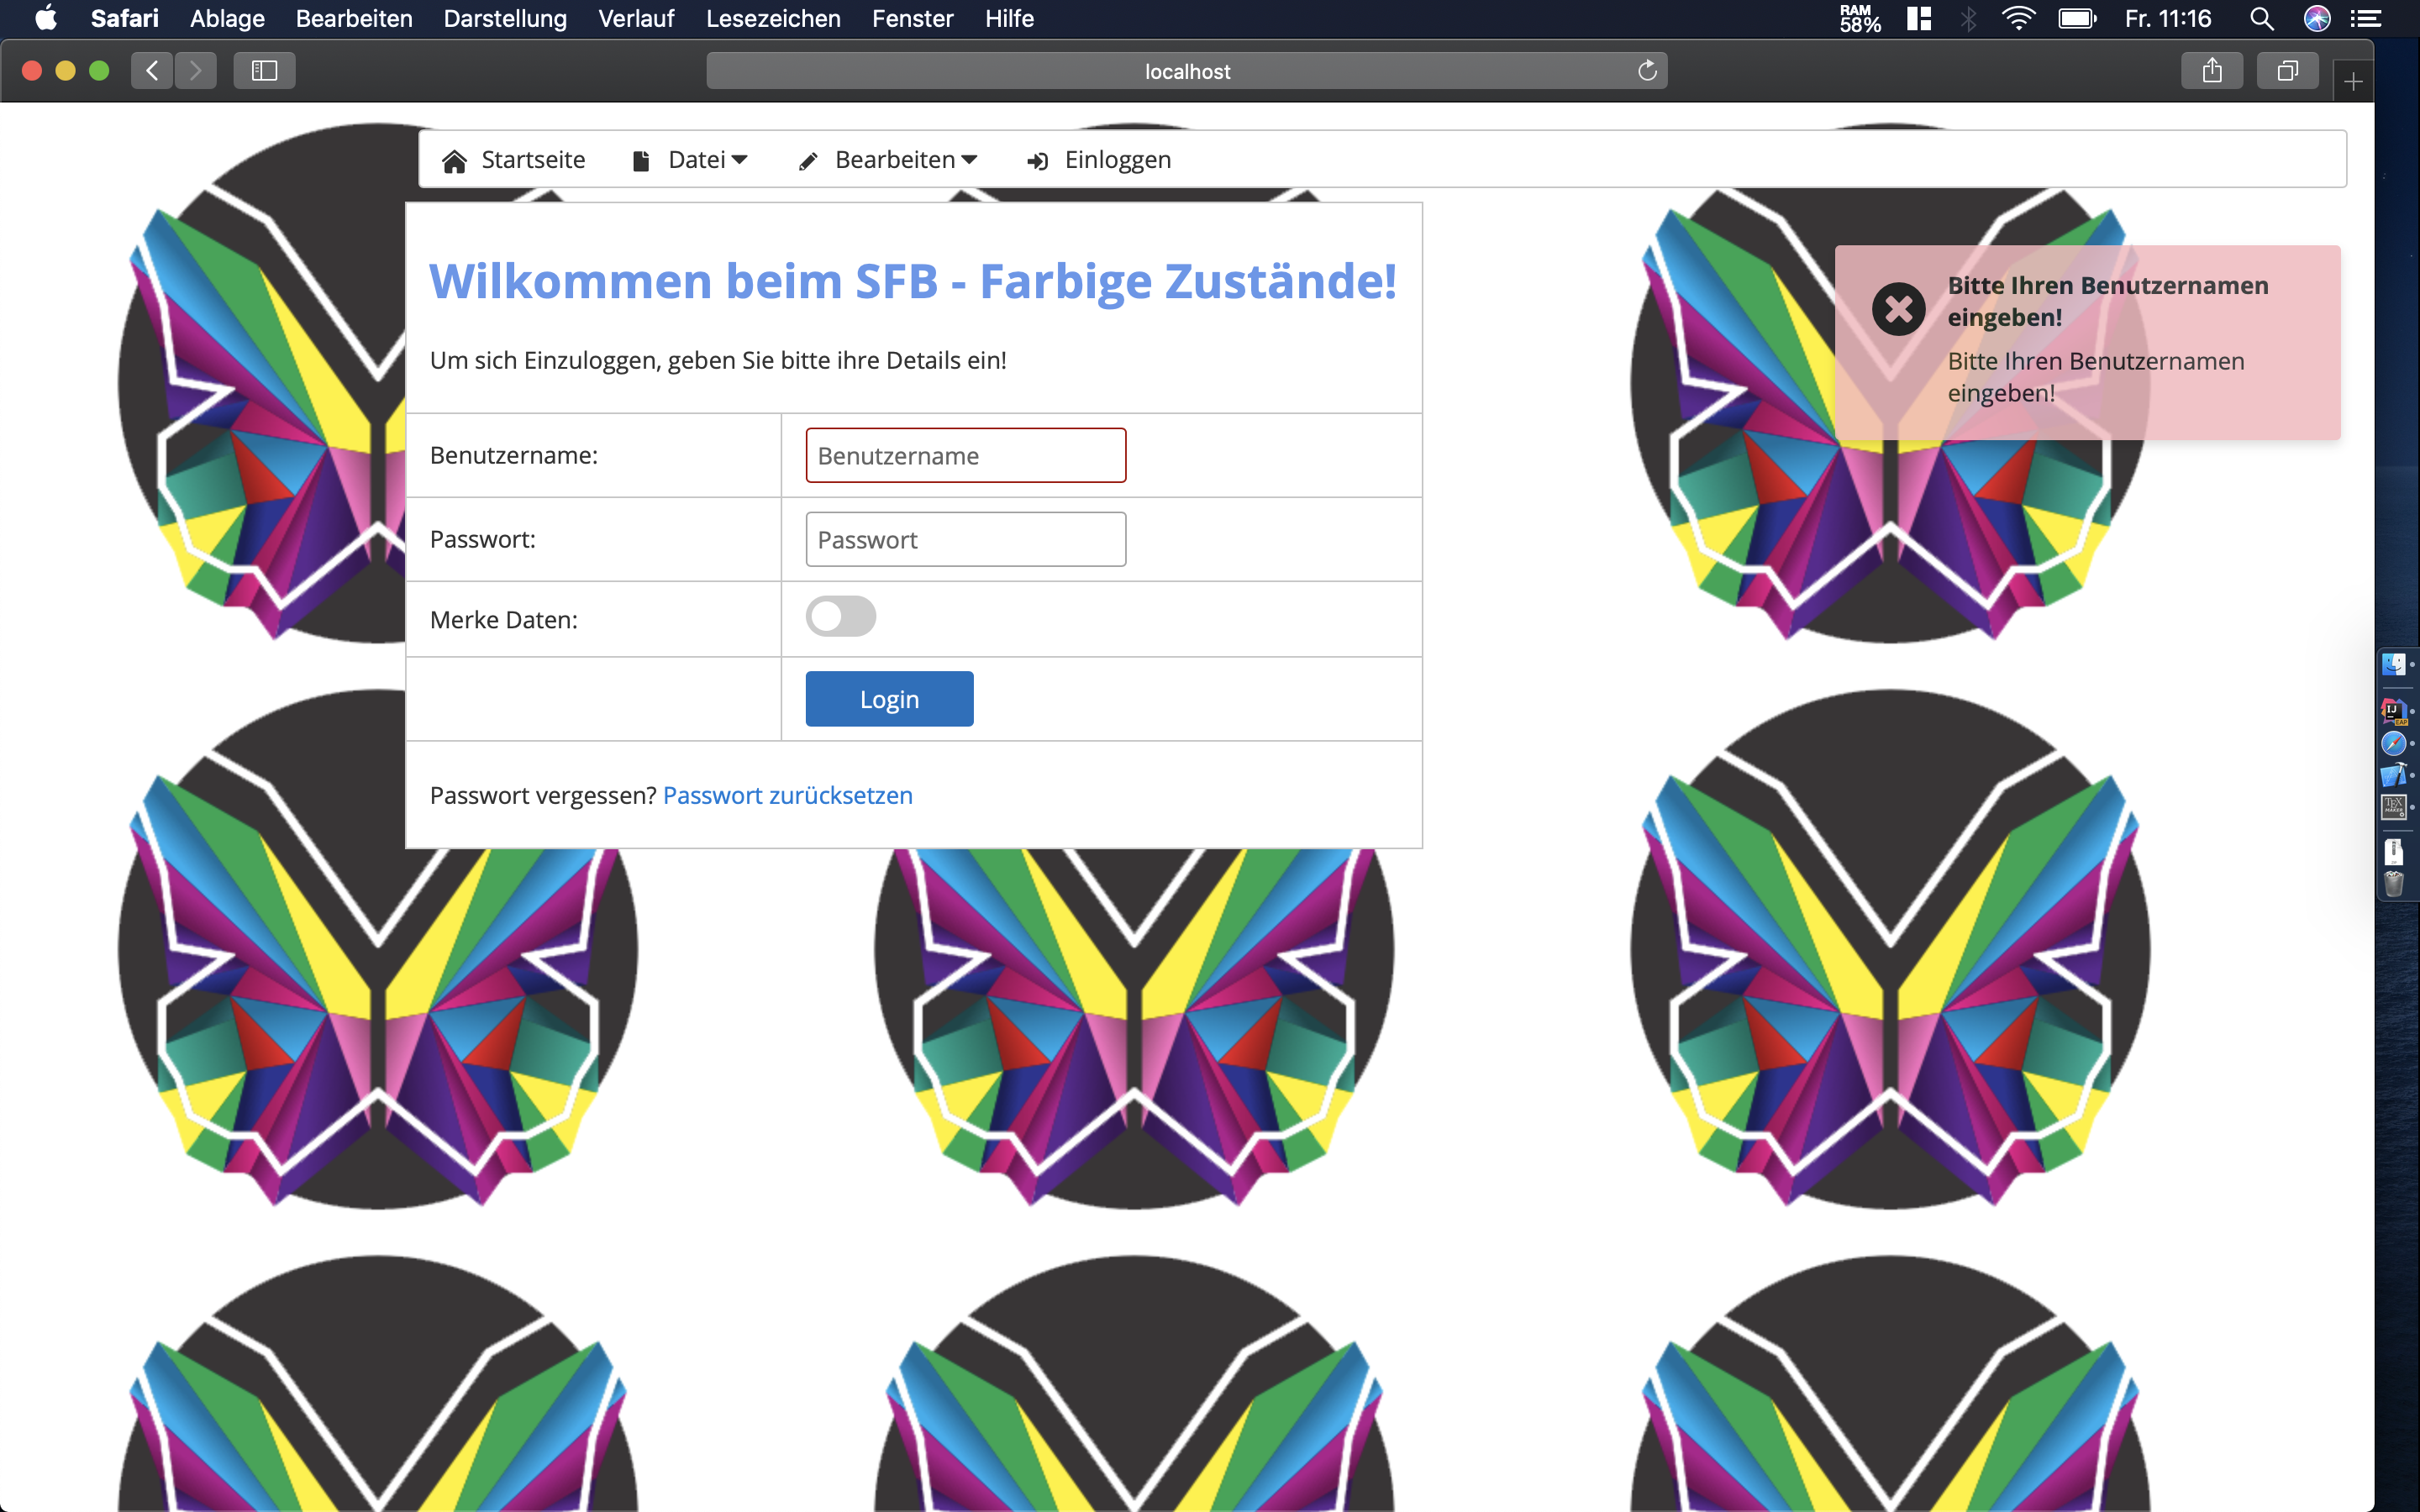
\includegraphics[width=1\textwidth]{Screenshots/311PasswordohneBenutzer.png}
\textit{Abbildung 3.1.1.7: password ohne Benutzer}
} \\
%%%Create User
%%Formular
\hypertarget{sc3.1.1.8}{
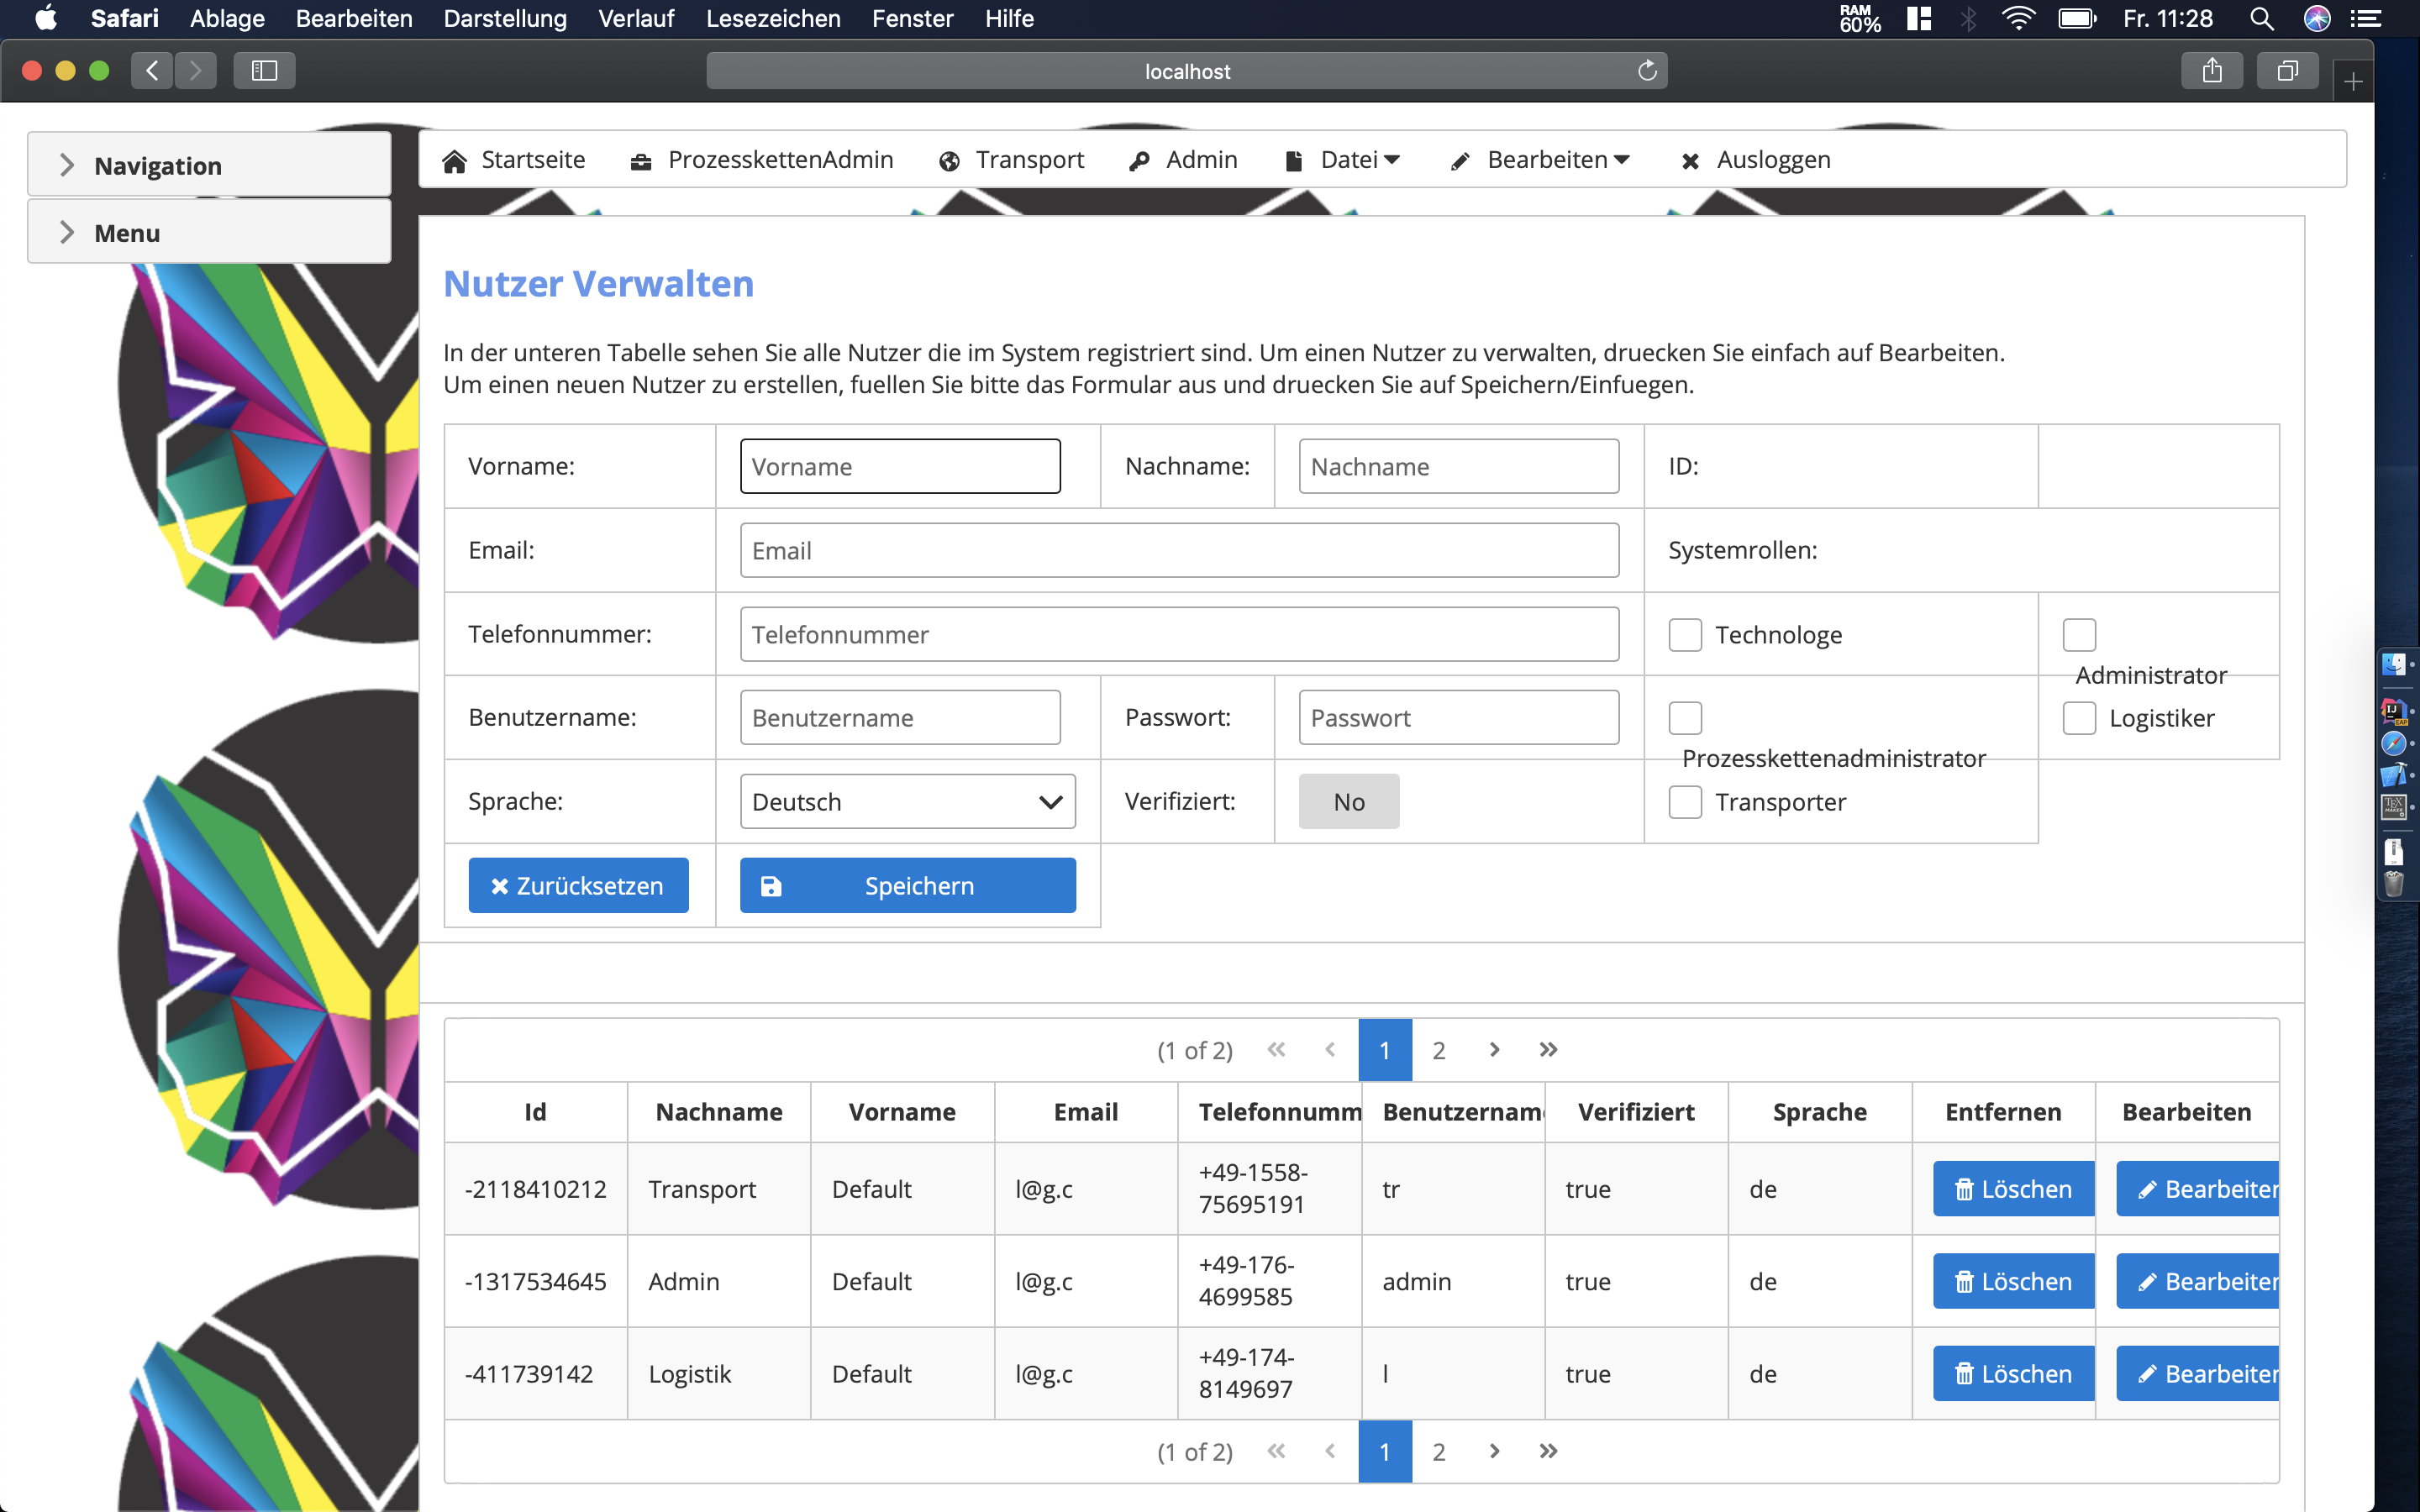
\includegraphics[width=1\textwidth]{Screenshots/UserErzeugenFormular.png}
\textit{Abbildung 3.1.1.8: Benutzer Formular and Tabelle von Benutzer}
} \\

%%InitialData
\hypertarget{sc3.1.1.9}{
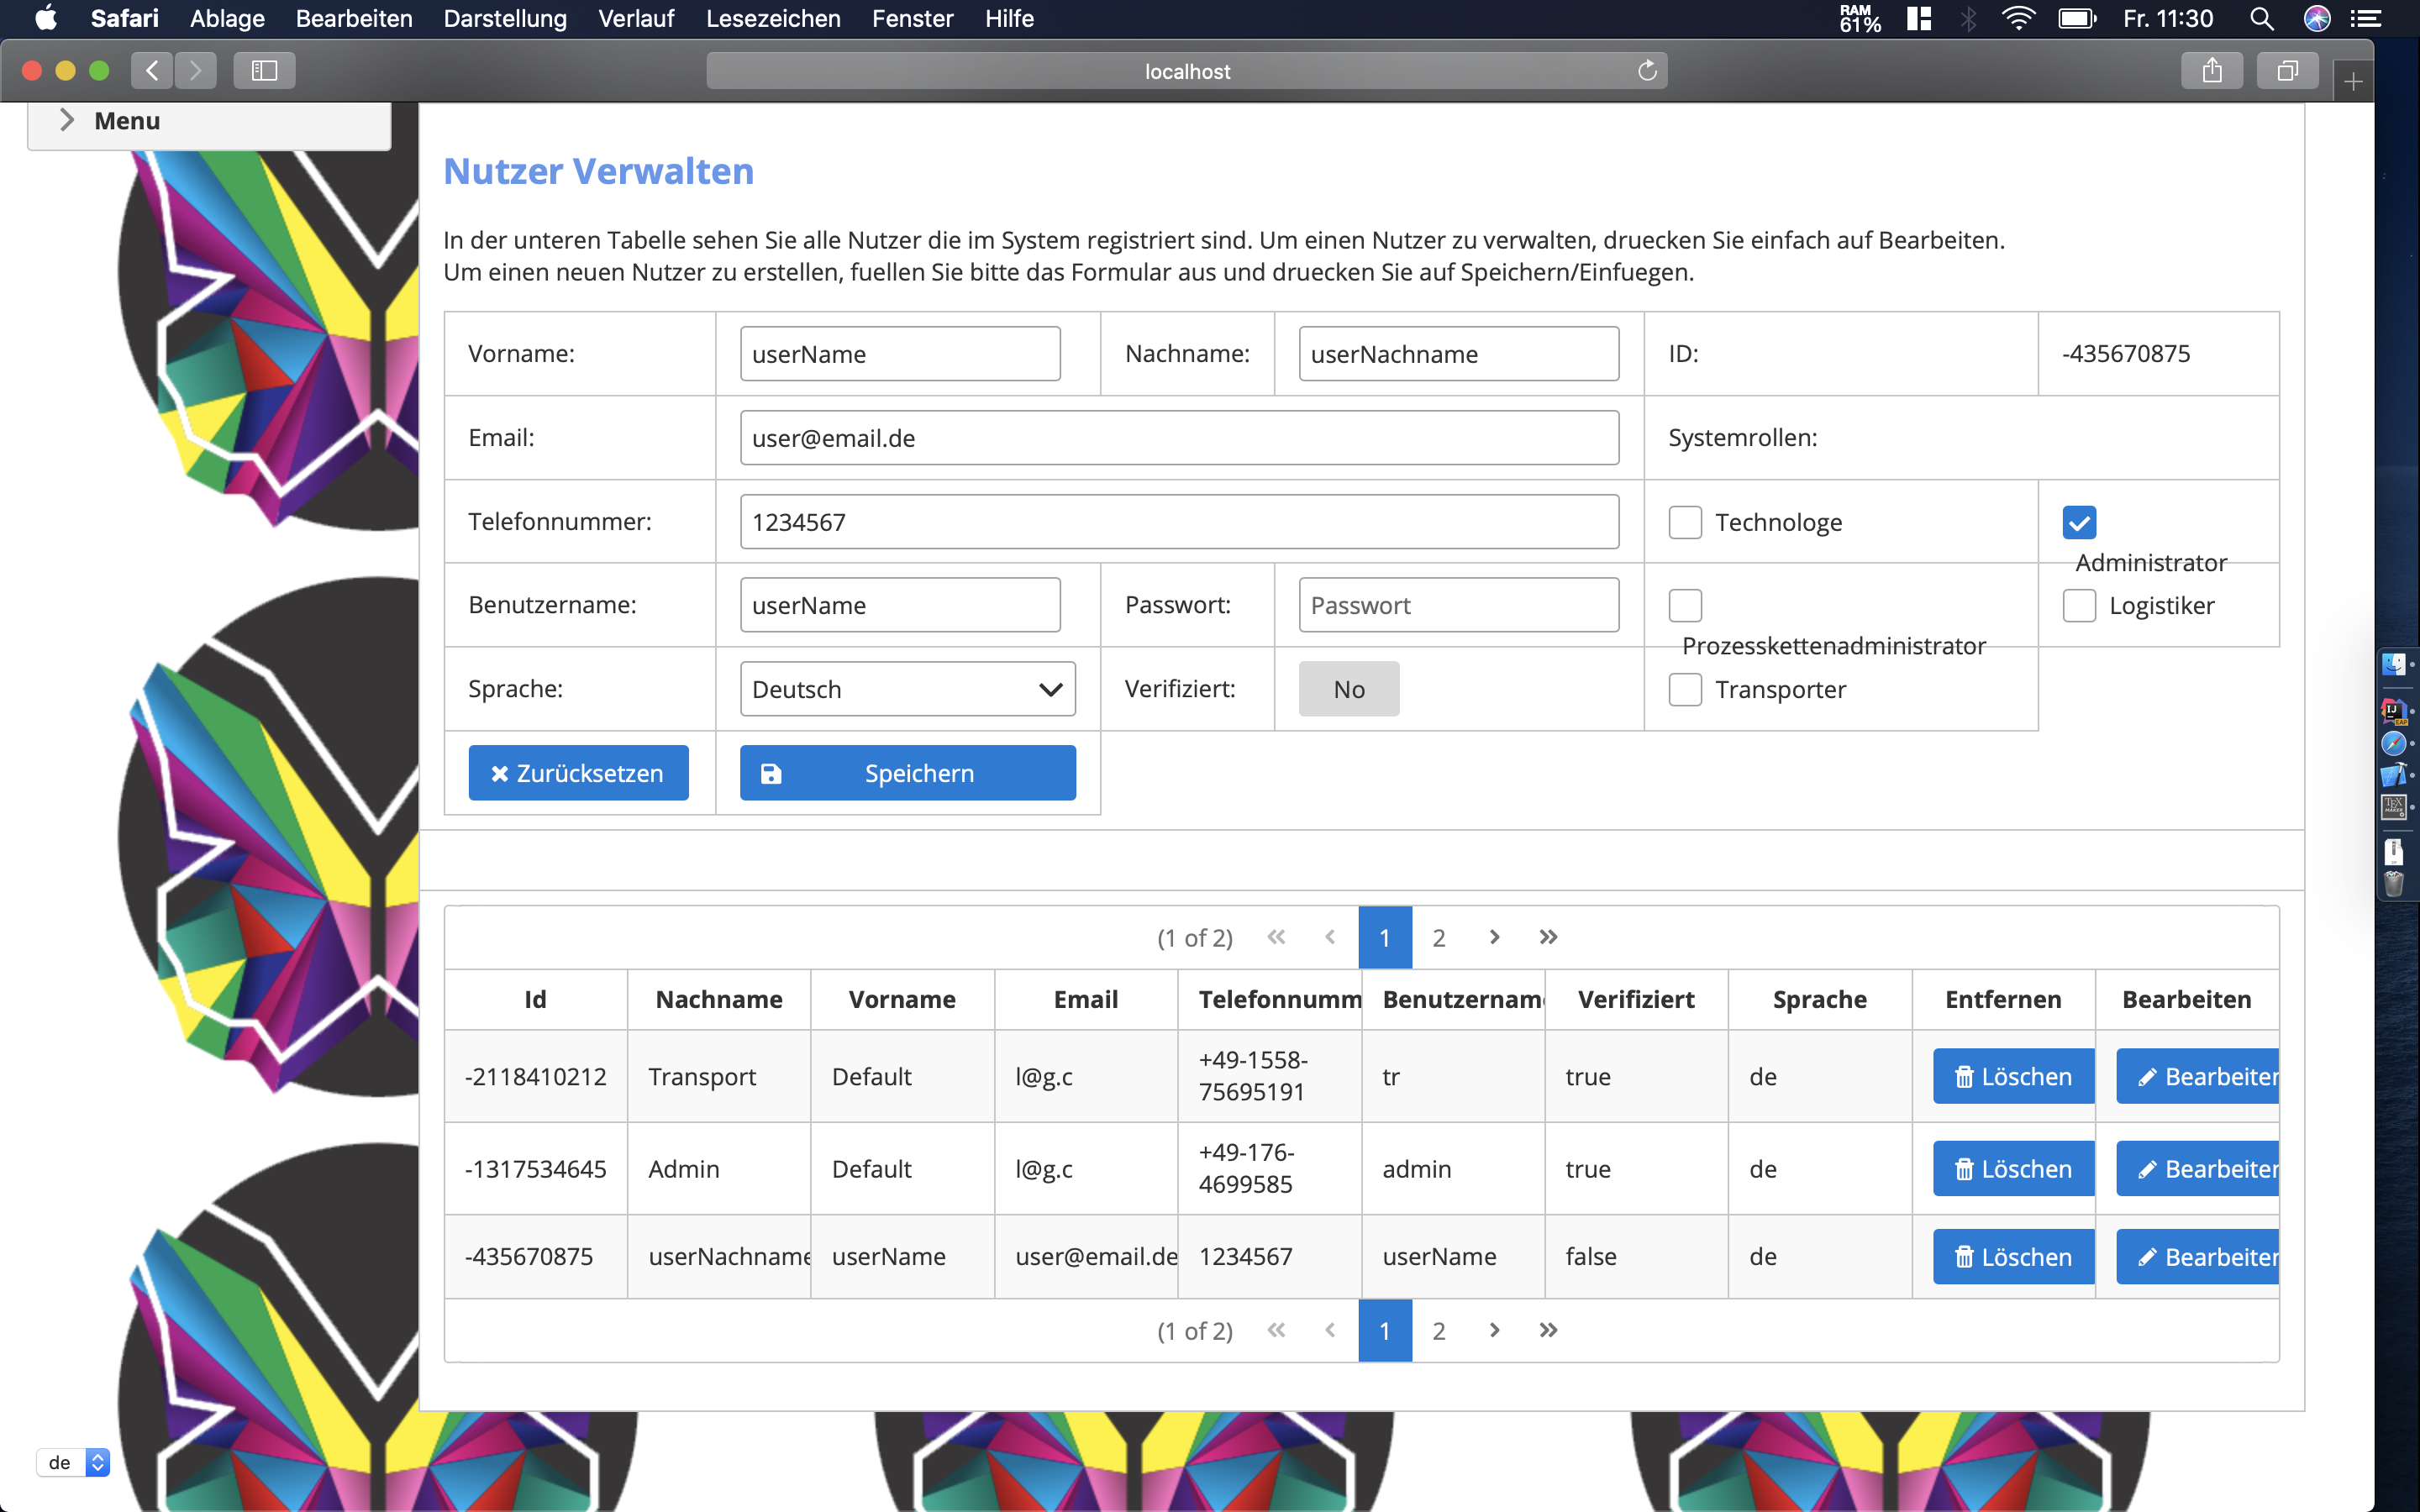
\includegraphics[width=1\textwidth]{Screenshots/userErzeugungInitialData.png}
\textit{Abbildung 3.1.1.9: Pruebe Data für ein neues Benutzer}
} \\

%%ErzeugunMeldung
\hypertarget{sc3.1.1.10}{
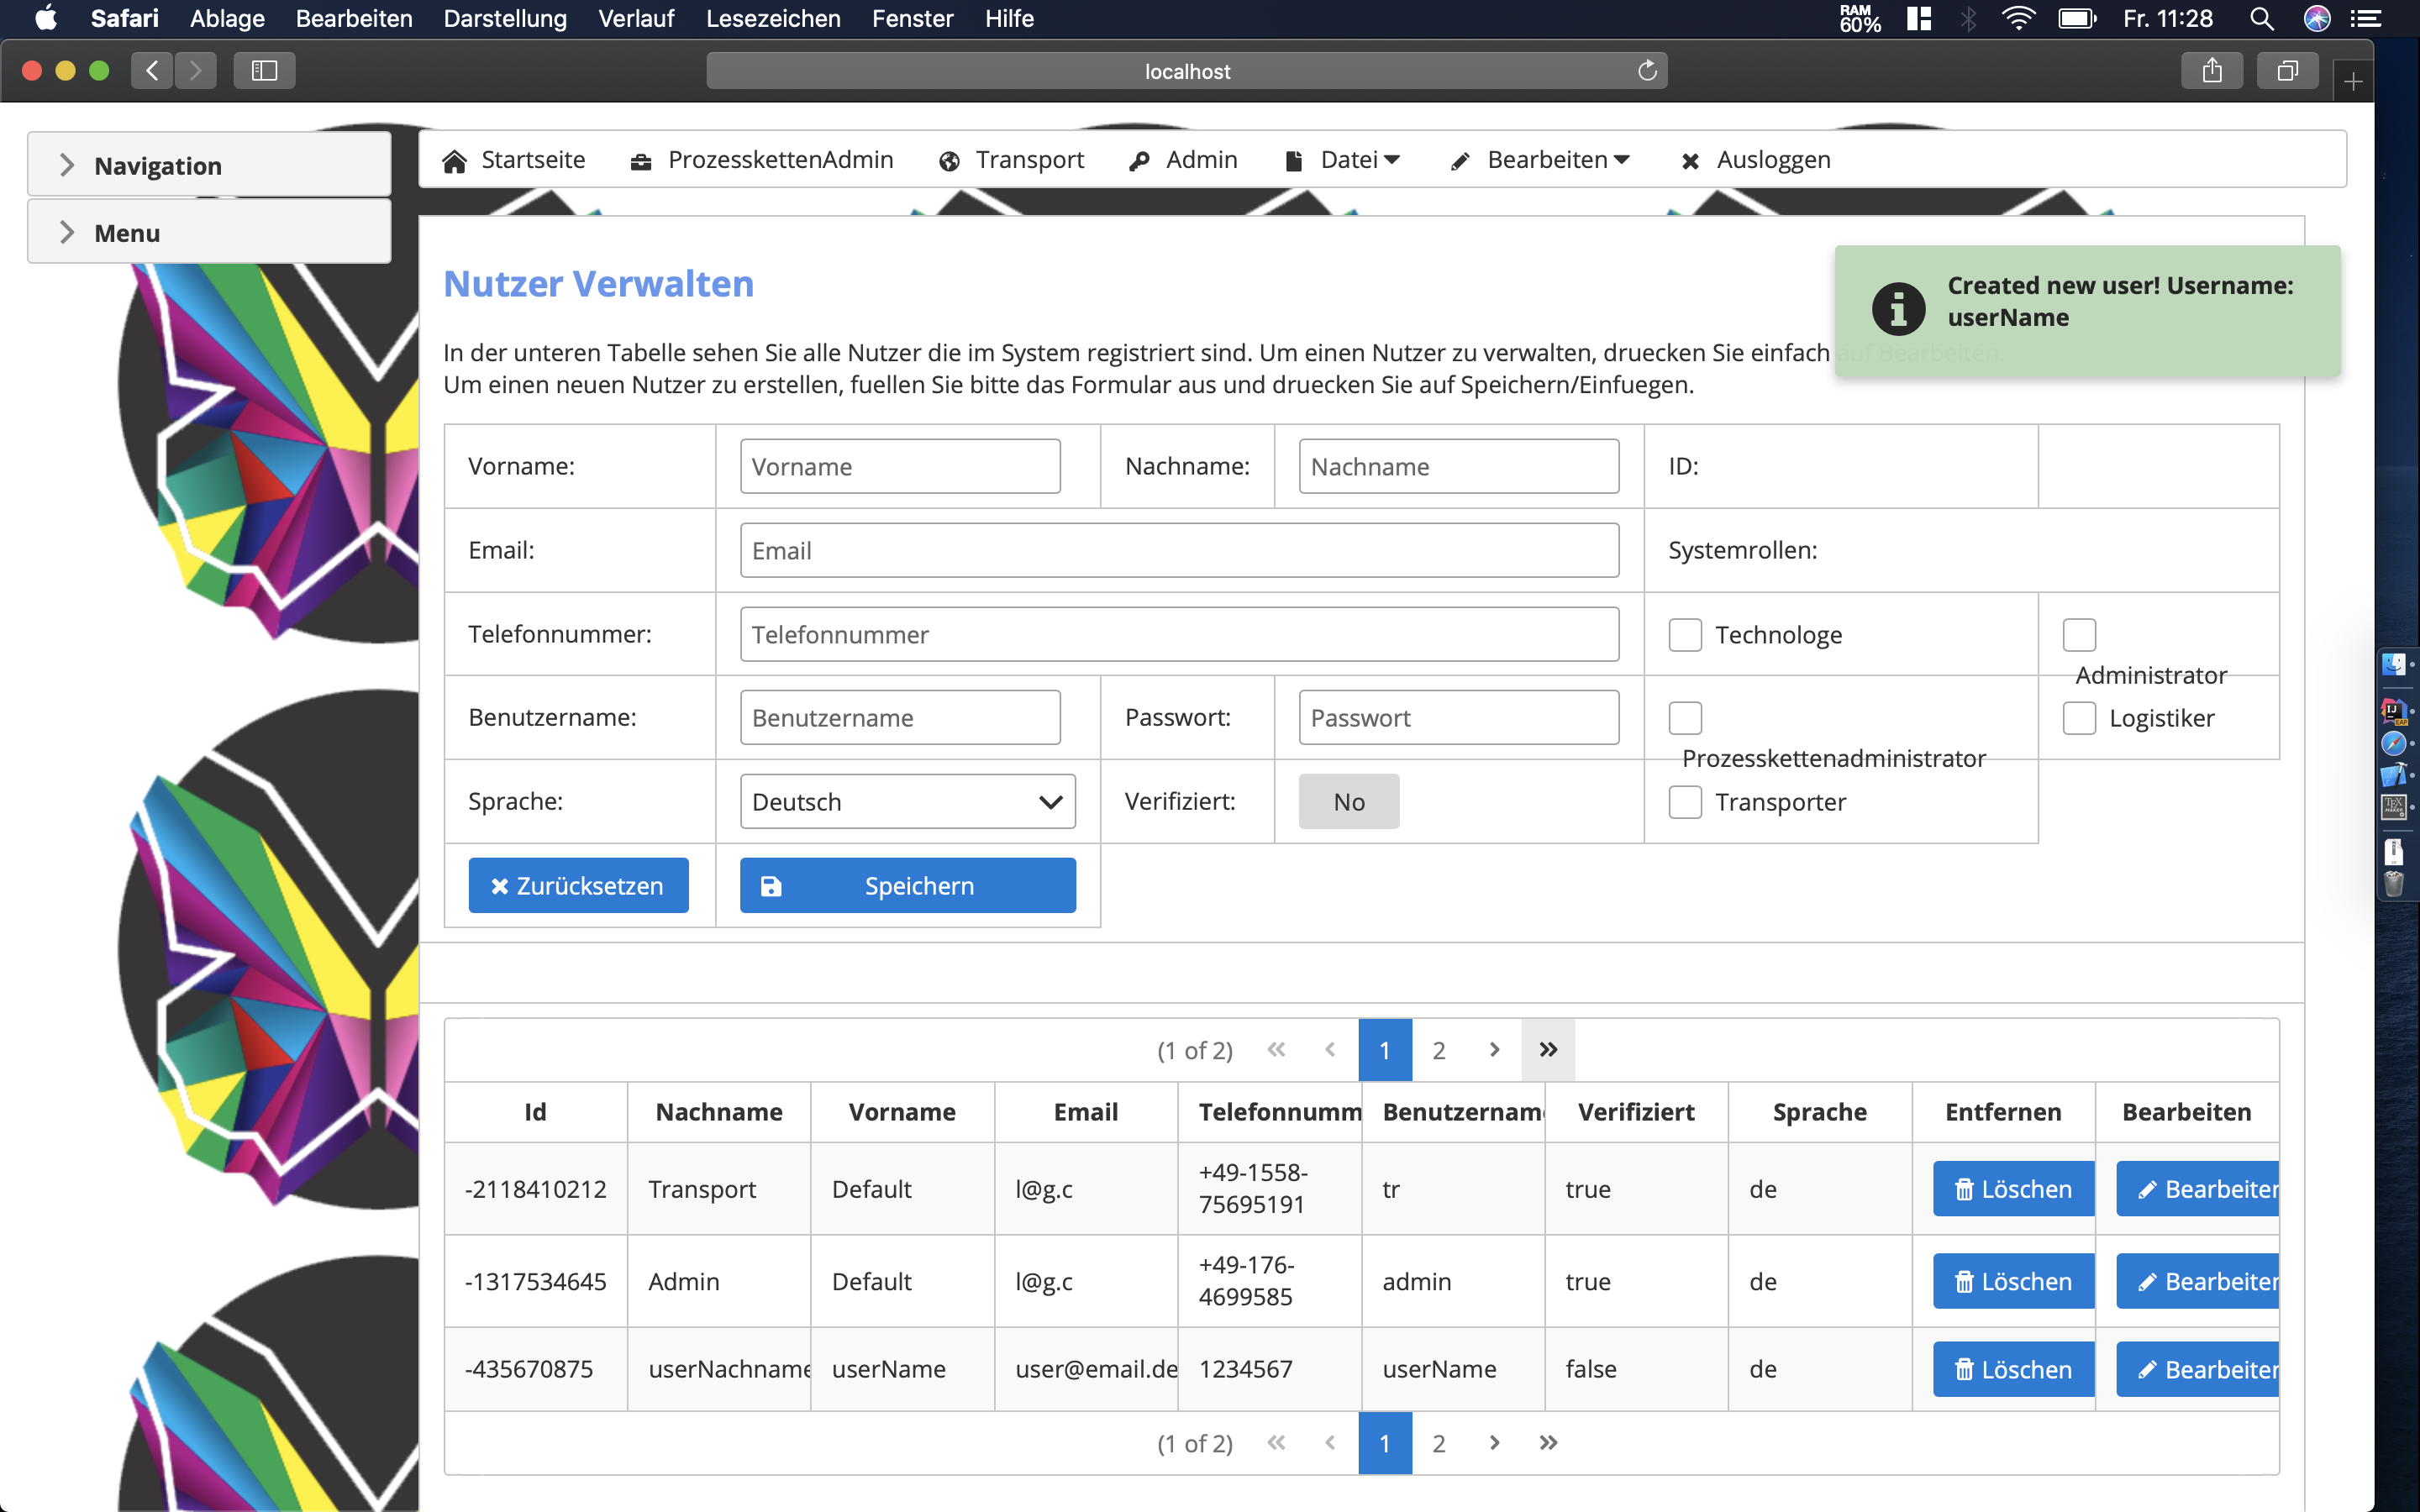
\includegraphics[width=1\textwidth]{Screenshots/userErzeugenMeldung.png}
\textit{Abbildung 3.1.1.10: Meldung von neuer Benutzer an der Webseite}
} \\

%%Bearbeiten
\hypertarget{sc3.1.1.11}{
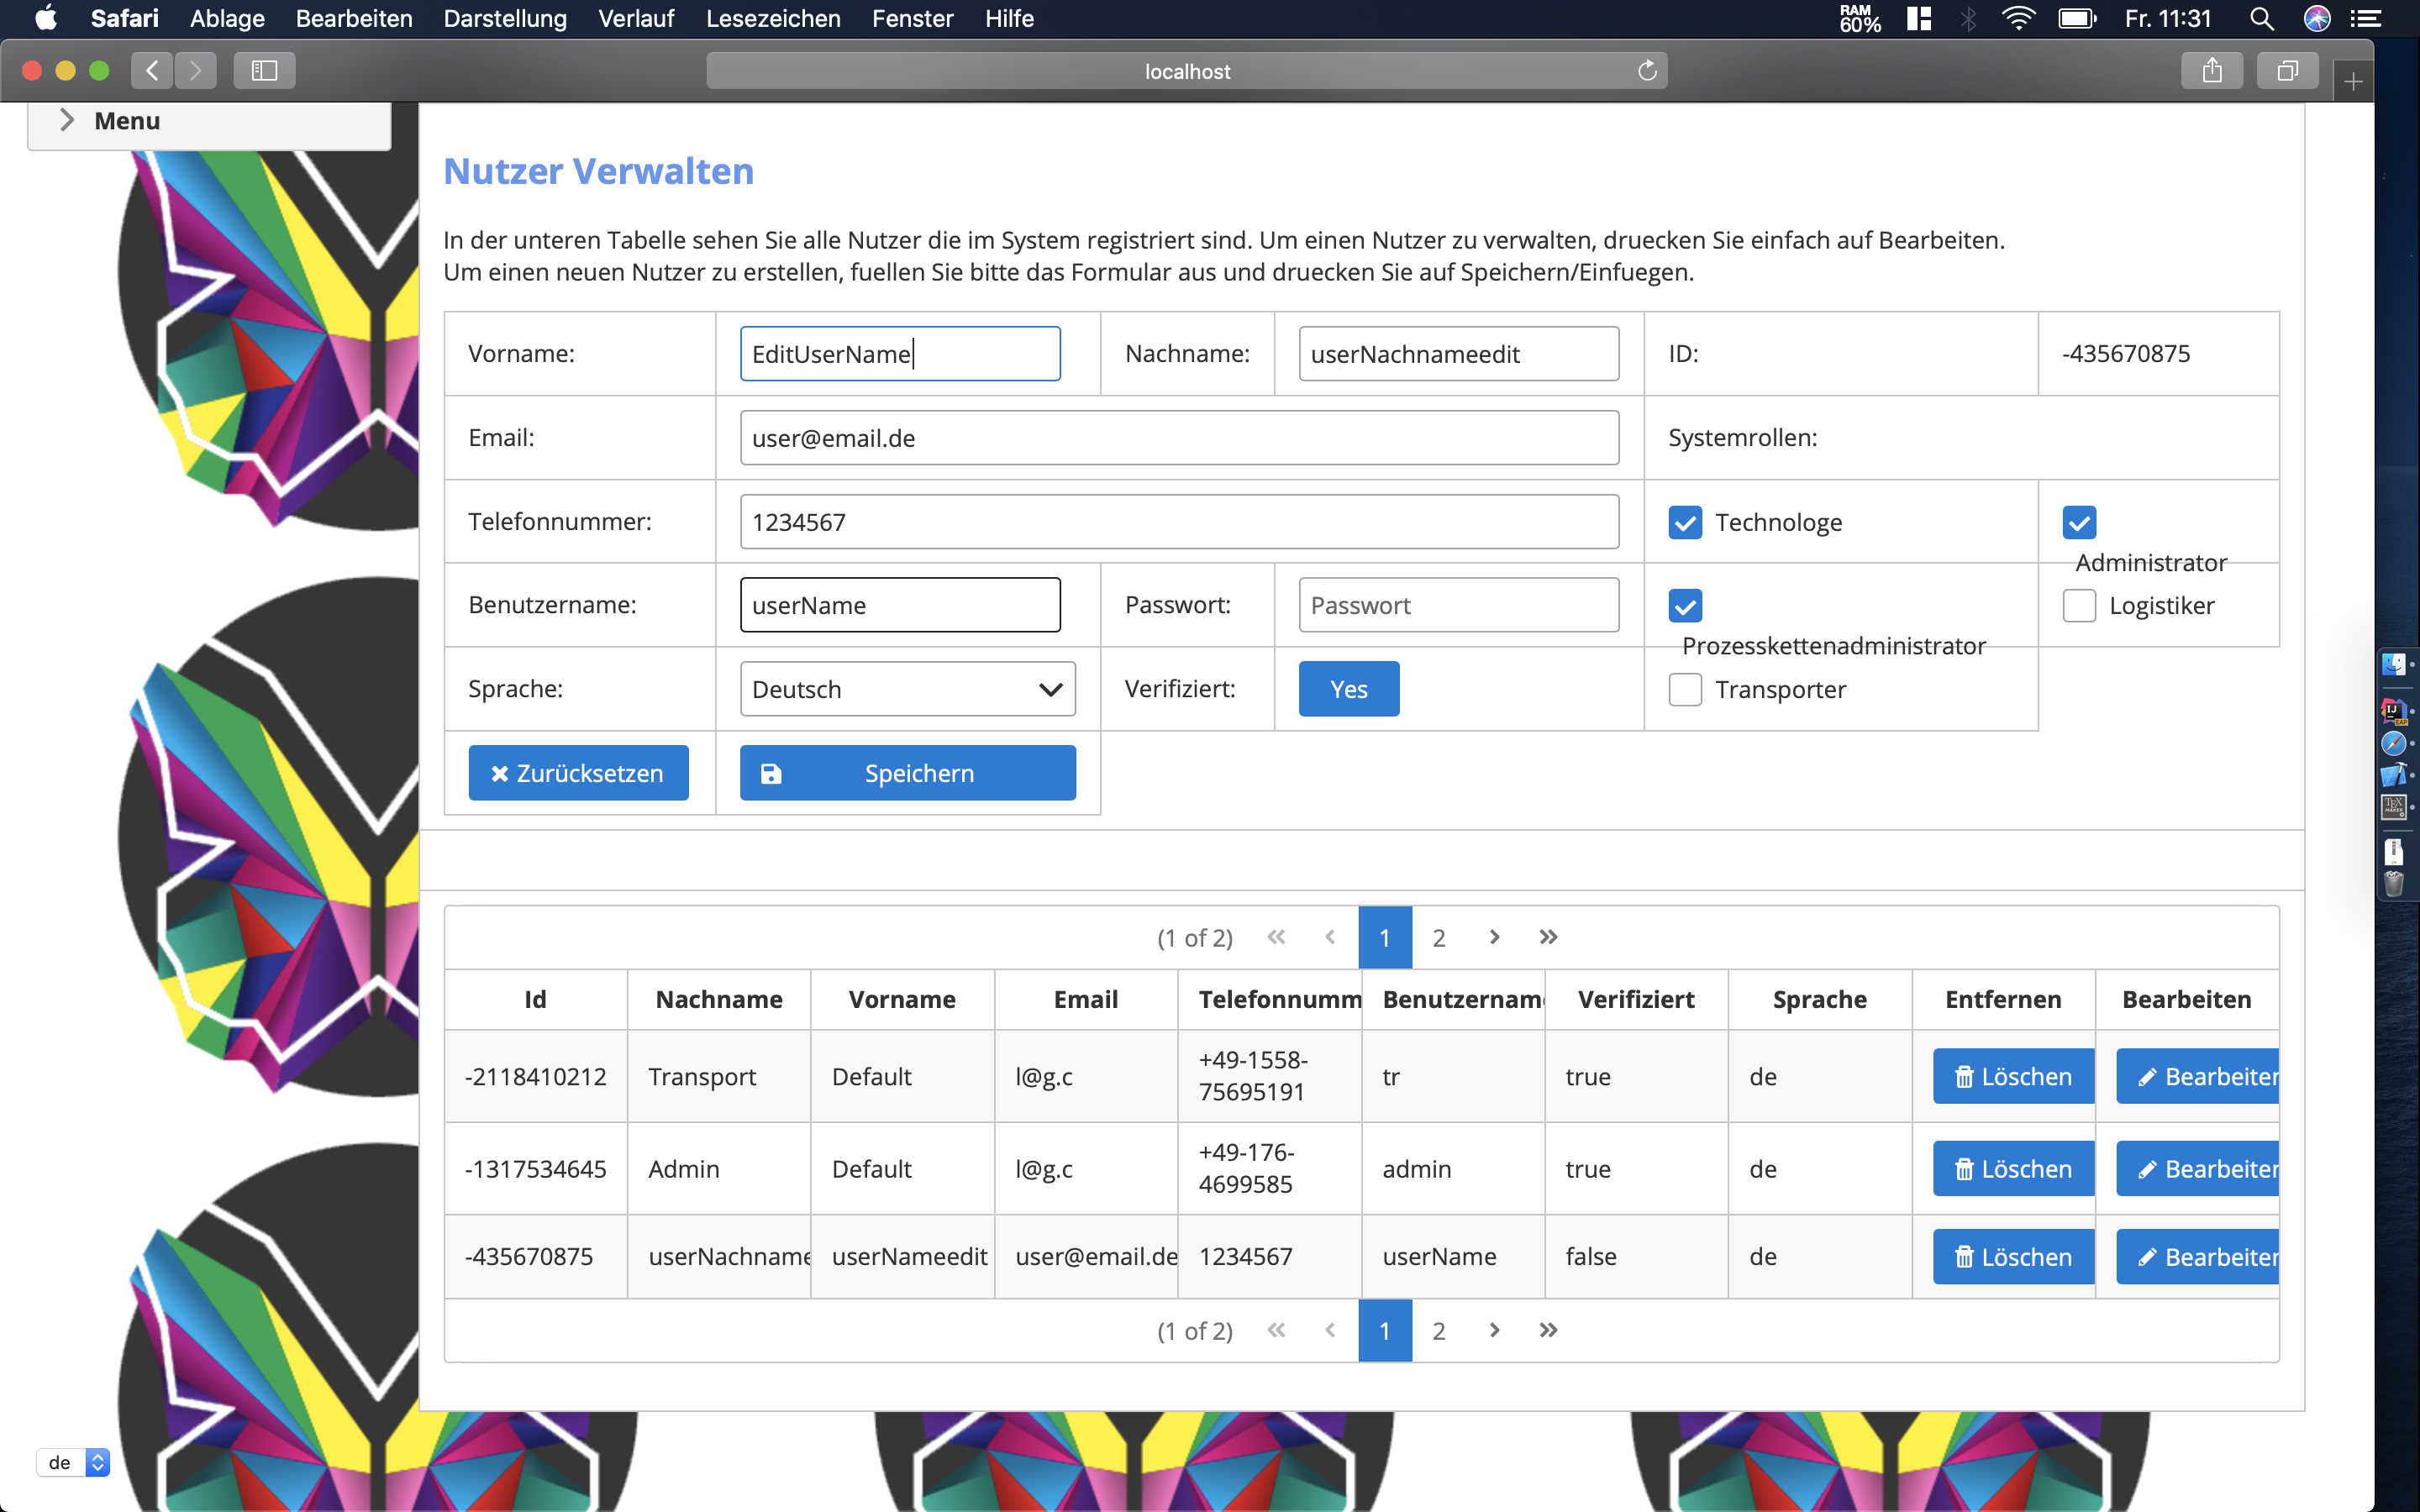
\includegraphics[width=1\textwidth]{Screenshots/UserEditData.png}
\textit{Abbildung 3.1.1.11: Bearbeitung von Data an der Pruebe Benutzer}
} \\

%%Editmeldung
\hypertarget{sc3.1.1.12}{
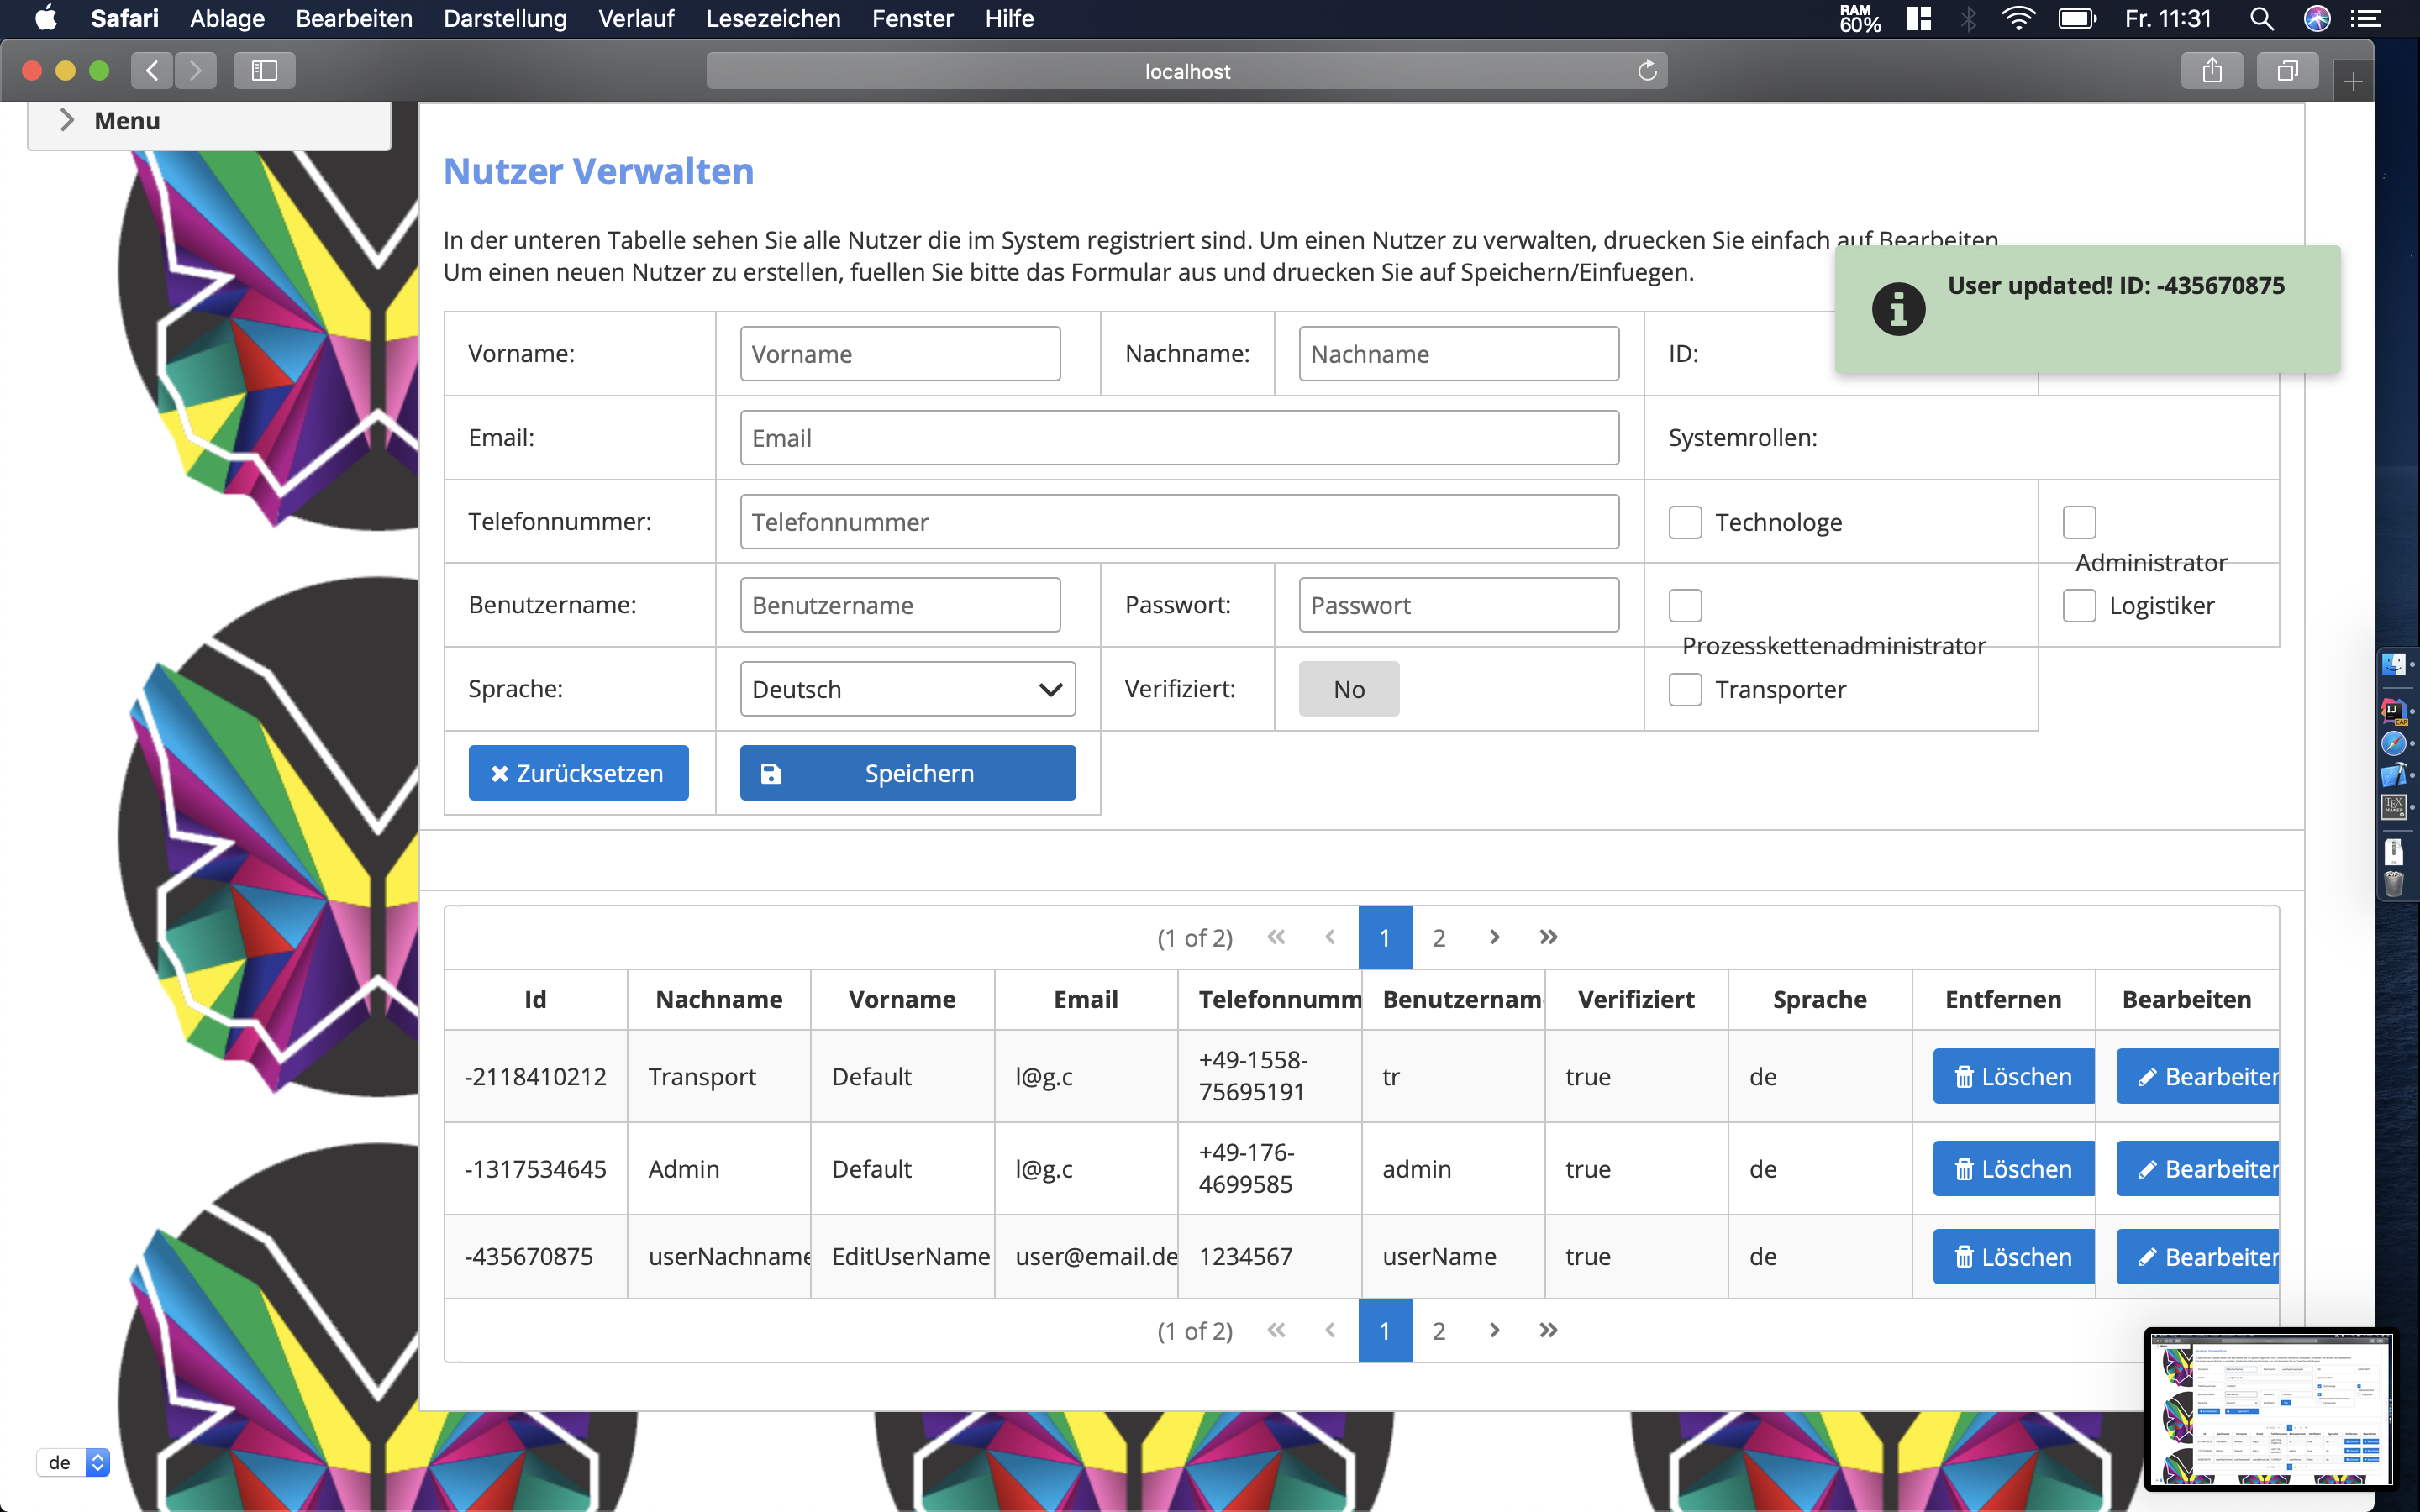
\includegraphics[width=1\textwidth]{Screenshots/editMeldung.png}
\textit{Abbildung 3.1.1.12: Meldung von Erfolgreiche Bearbeitung der Data von nutzer}
} \\
%%InconsistenceData
\hypertarget{sc3.1.1.13}{
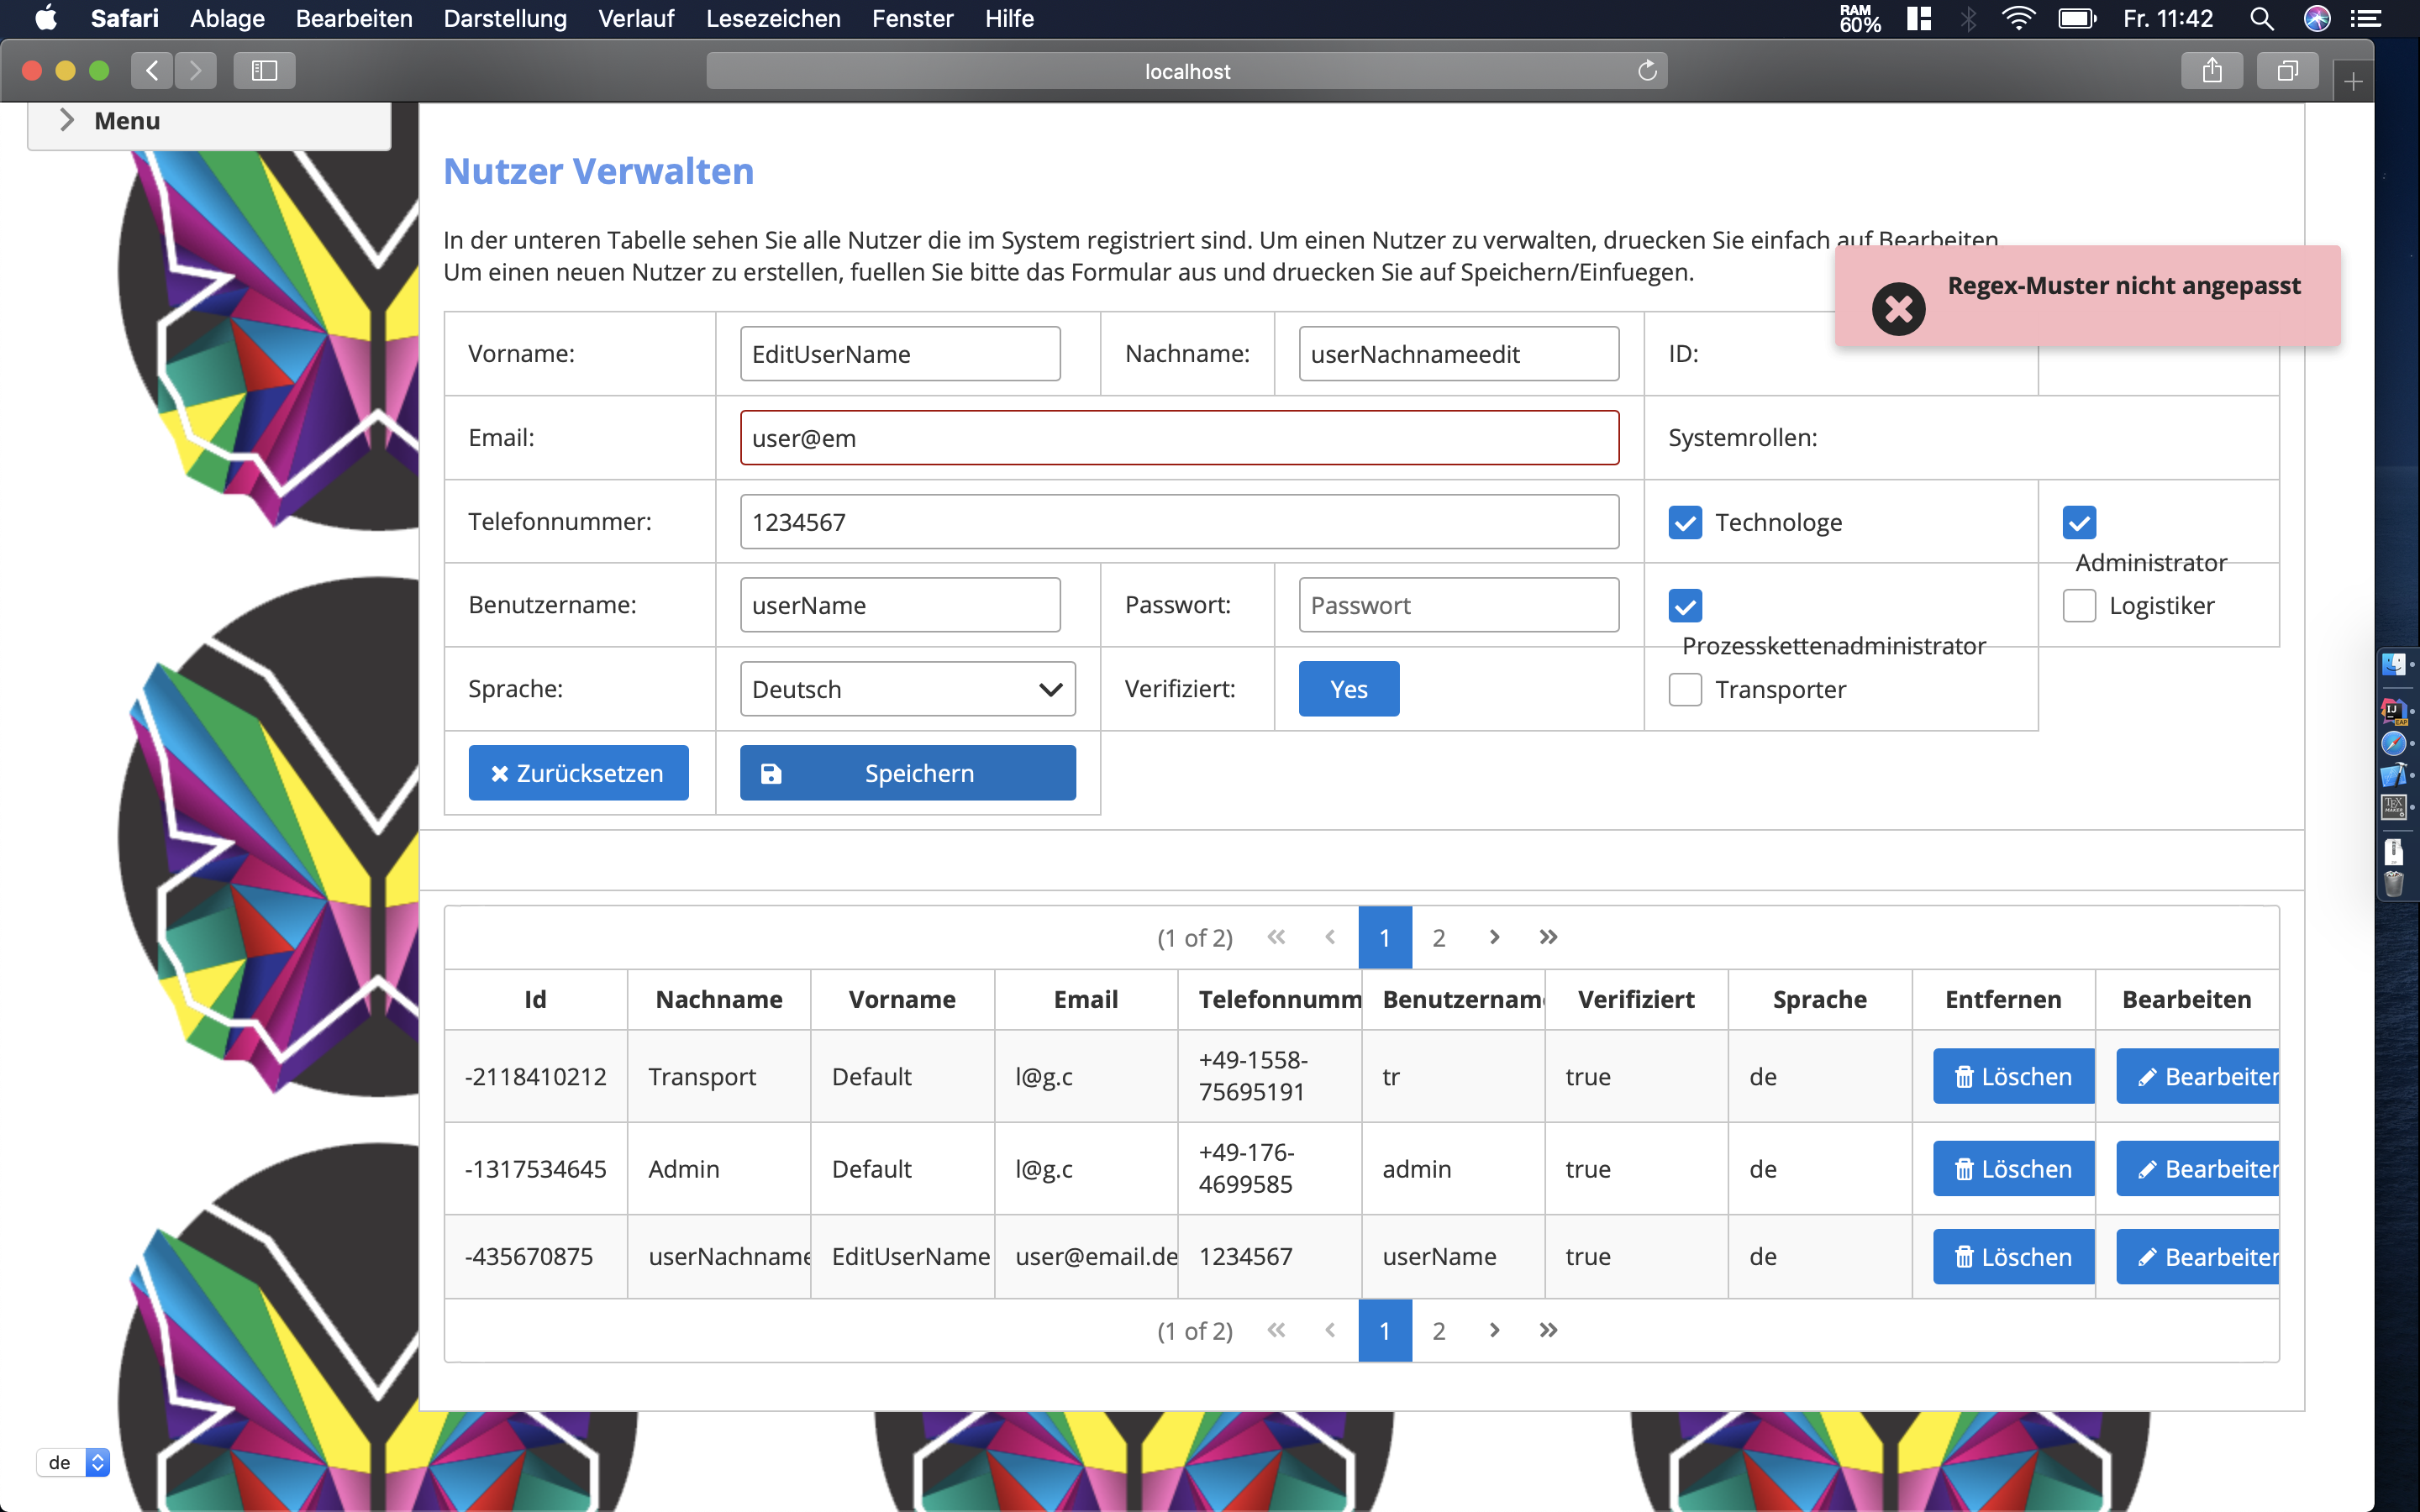
\includegraphics[width=1\textwidth]{Screenshots/InconsistenceDataUserBearbeitung.png}
\textit{Abbildung 3.1.1.13: Meldung von Erfolgreiche Bearbeitung der Data von nutzer}
} \\

\color{red} Es muss noch mit falschem Benutzernamen getestet werden!

%%

\subsubsection{Anwendungsfall: Beispiel 2}

%%

\subsubsection{Anwendungsfall: Beispiel 3}

%%

\subsubsection{Anwendungsfall: Beispiel 4}

%%

\subsubsection{Anwendungsfall: Beispiel 5}

%%%%%%%%%%%%

\subsection{Automatisierte Funktionstests}

\subsubsection{Anwendungsfall: Beispiel 1}

%%

\subsubsection{Anwendungsfall: Beispiel 2}

%%

\subsubsection{Anwendungsfall: Beispiel 3}

%%

\subsubsection{Anwendungsfall: Beispiel 4}

%%

\subsubsection{Anwendungsfall: Beispiel 5}

%%%%%%%%%%%%%%%%%%%%%%%%%%%%%%%%%%%%%%%%%%%%%%%%%%%%%%%%%%%%%%%%%%%%%%%%

\end{document}














